\chapter{Usability and Performance Validation} \label{cha:analysis}

In this chapter the performance and usability of the \textbf{Hybrid Fortran} framework will be verified. For this reason, a sample implementation with a subset of the ASUCA physical core's functionality has been implemented. Sec.~\ref{sec:asucaRadImplementation} will give an idea of the scope of this implementation. Sec.~\ref{sec:usabilityValidation} will examine the usability of \textbf{Hybrid Fortran} compared to OpenACC when applied to the ASUCA physical process. Sec.~\ref{sec:performanceValidation} will offer an examination of the performance of the current CPU and GPU implementations that are being applied with \textbf{Hybrid Fortran} in comparison to the performance of OpenACC as well as code that has been optimized specifically for the CPU.

\section{Scope of Sample ASUCA Implementation} \label{sec:asucaRadImplementation}

\begin{figure}[htpb]
        \centering
        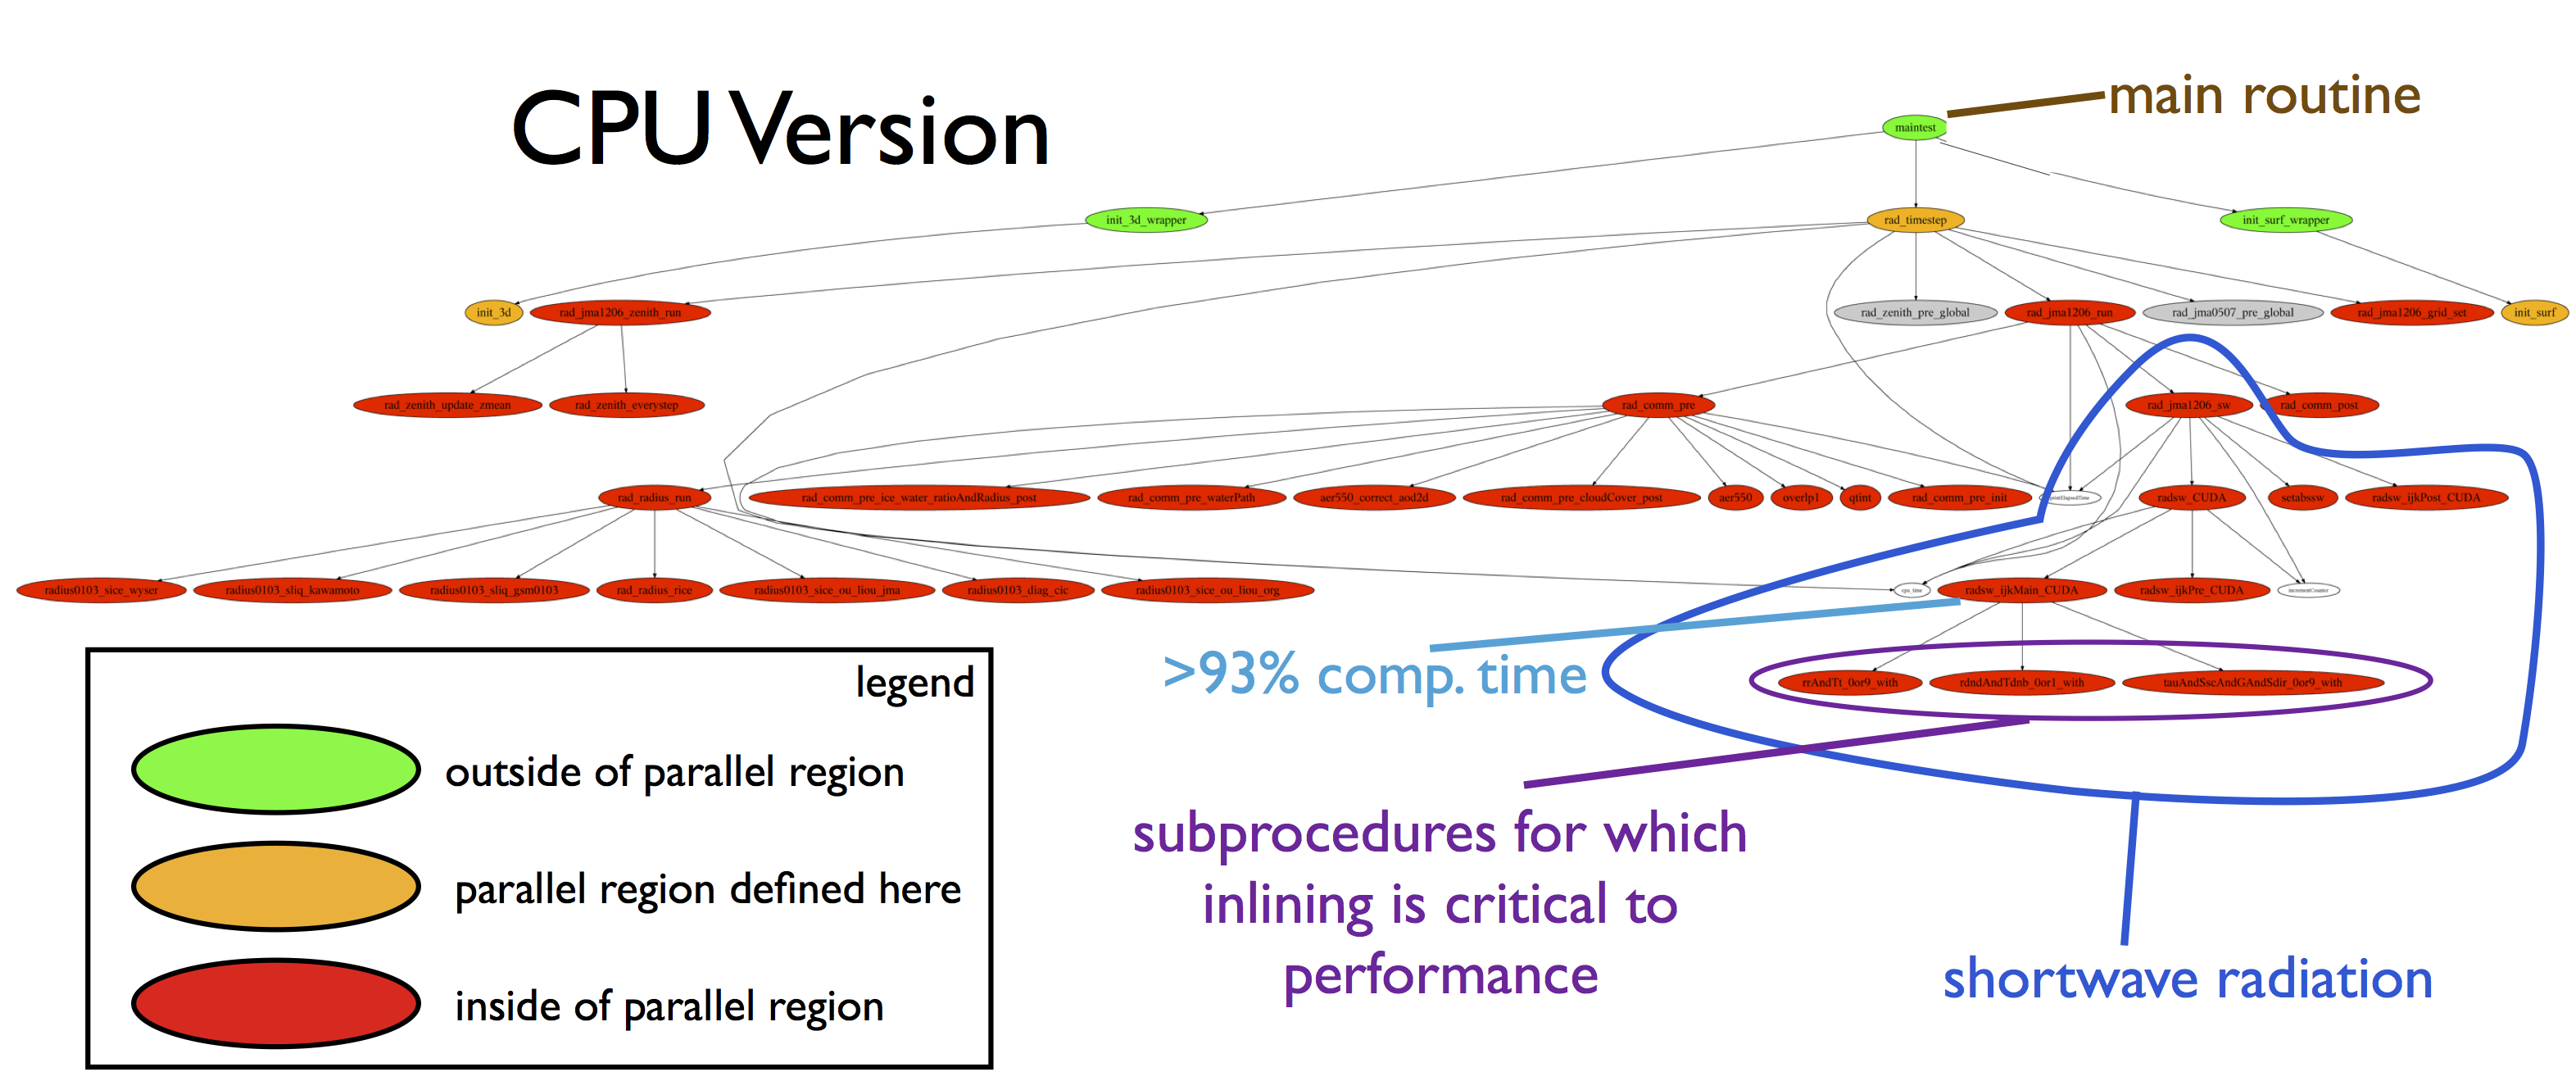
\includegraphics[width=14cm]{figures/asucaPPImplementationCPU}
        \caption[CPU Version of Sample Hybrid Fortran Implementation]{Overview CPU version of ASUCA sample implementation.}
        \label{figure:asucaPPImplementationCPU}
\end{figure}

\begin{figure}[htpb]
        \centering
        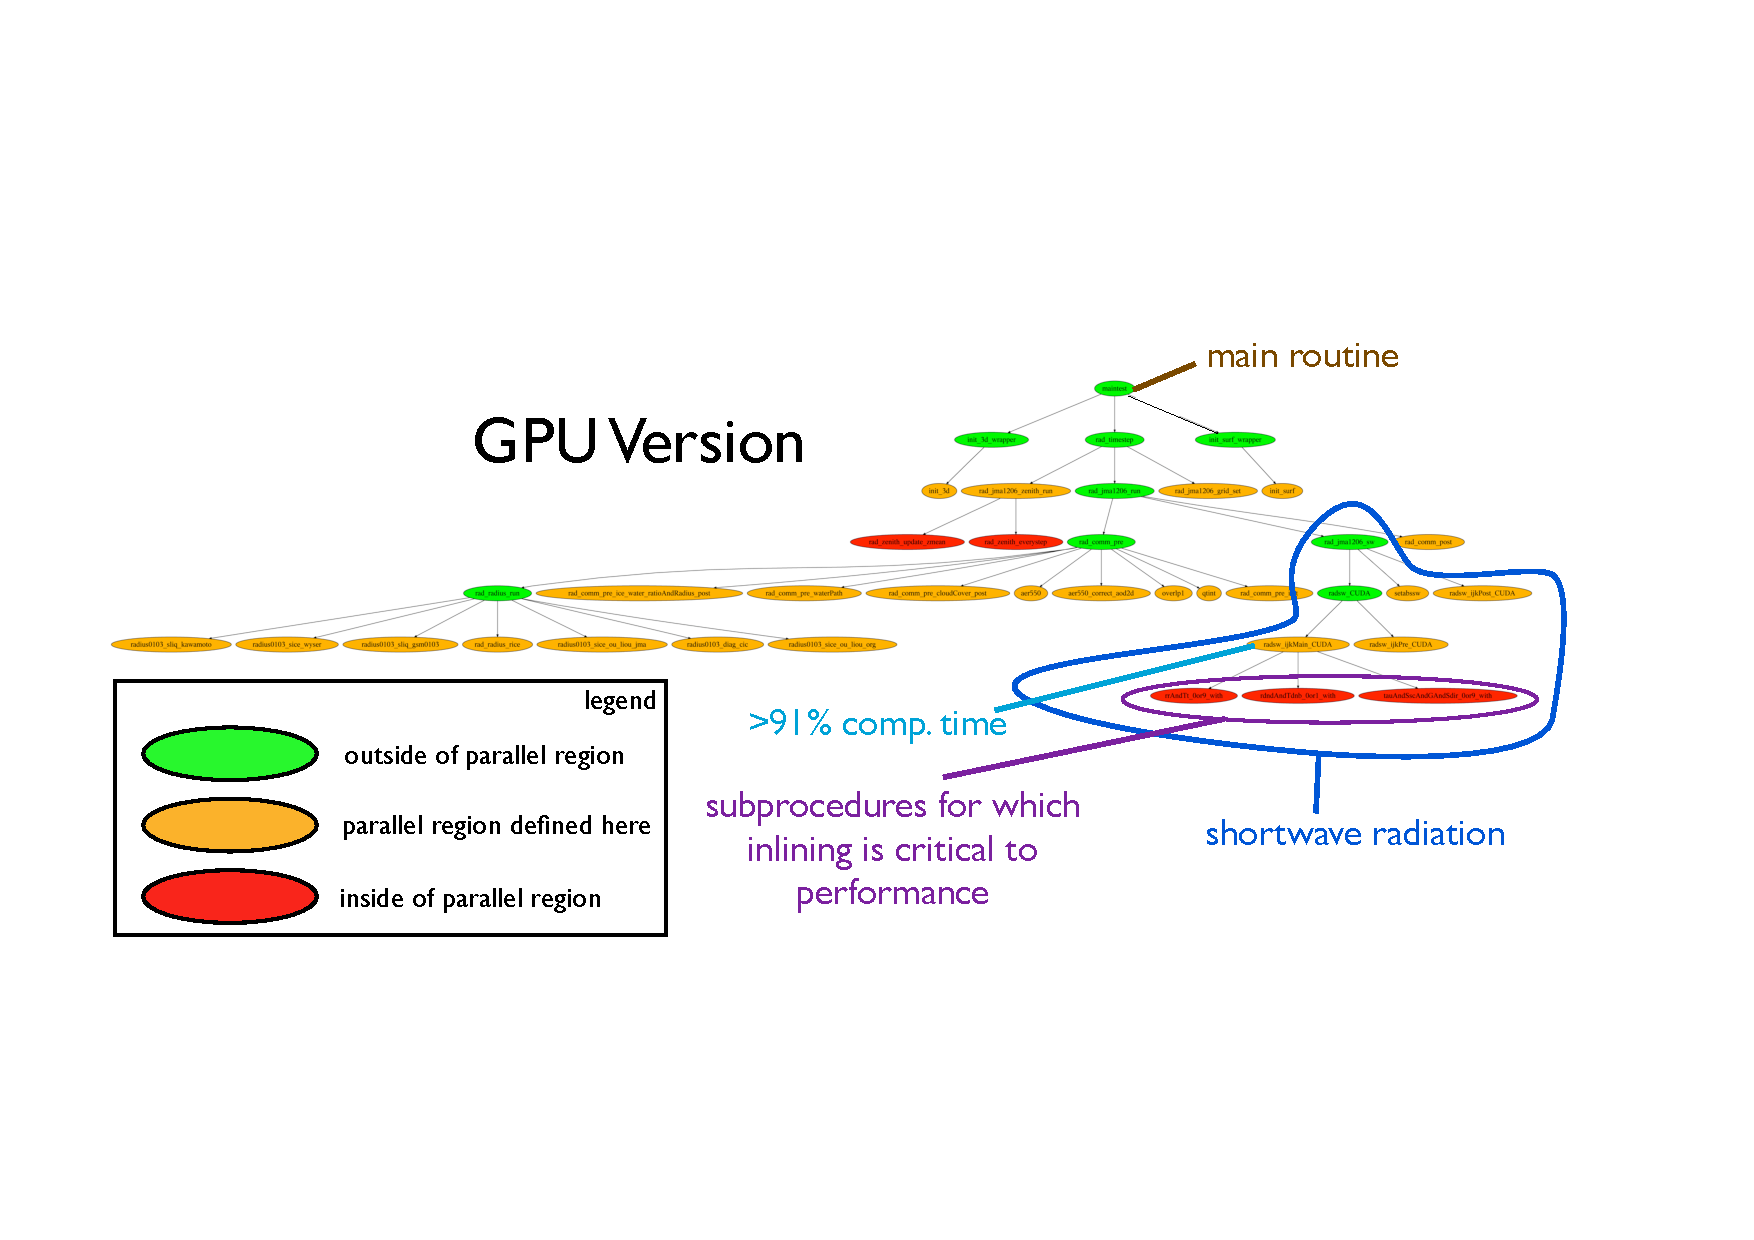
\includegraphics[width=14cm]{figures/asucaPPImplementationGPU}
        \caption[GPU Version of Sample Hybrid Fortran Implementation]{Overview GPU version of ASUCA sample implementation.}
        \label{figure:asucaPPImplementationGPU}
\end{figure}

Fig.~\ref{figure:asucaPPImplementationCPU} and fig.~\ref{figure:asucaPPImplementationCPU} show the scope of the sample ASUCA implementation\footnote{The automatical graphical callgraph representation has been used here. This can be created by running ``make graphs'' in the project directory.}. Essentially all routines necessary for the ASUCA radiation module have been implemented with the exception of longwave radiation. These figures allow the following observations:

\begin{enumerate}
 \item The CPU ``sees'' three loops over the \verb|IJ| domains (orange nodes) - two for initialisations and one for the actual timestep computation.
 \item The GPU on the other hand sees 23 loops over the \verb|IJ| domains, i.e. 23 CUDA kernels are being created.
 \item One kernel, which is part of the shortwave radiation module, is responsible for over 93\% of this implementation's computation time when executed on CPU and over 91\% when executed on GPU.
 \item The extent of the shortwave radiation module is indicated by the blue marking. This module has also been benchmarked using OpenACC as well as manual CUDA Fortran, as discussed in cha.~\ref{cha:evaluation}, hence its performance will be analyzed more closely in sec.~\ref{sec:performanceValidation}).
 \item The violet marking shows three additional scalar subroutines (compared to the original code version) that have been introduced as a GPU optimization. The performance impact of their inlining will also be discussed in sec.~\ref{sec:performanceValidation}.
\end{enumerate}

\clearpage
\section{Usability of Hybrid Fortran versus PGI OpenACC} \label{sec:usabilityValidation}

In order to examine the usability differences between \textbf{Hybrid Fortran} and PGI OpenACC\footnote{Because of difficult usability in the tested version of HMPP OpenACC and given time constraints of this thesis, it has been decided not to pursue a HMPP implementation for the shortwave submodule. See also sec.~\ref{sub:hmppVsPGIUsability}.} we will examine the code changes necessary for the portation of an example subroutine. The \verb|abssw| subroutine from the shortwave submodule has been chosen with the following criteria:

\begin{enumerate}
 \item The data access patterns as well as the amount of computations per data array is representative for the ASUCA physical processes.
 \item The subroutine is large enough to show typical code complexity, yet is small enough to be shown here.
\end{enumerate}

Please note, however, that this subroutine's execution time is a small fraction of the radiation module's overall execution time.

We define two classes of source code modifications as follows:

\begin{description}
 \item [Green Code Modification]: \begin{enumerate}
    \item New code lines.
    \item Code edits using a trivial find/replace operation over the entire routine (no regular expressions are necessary).
  \end{enumerate}
 \item [Yellow Code Modification]: \begin{enumerate}
    \item Code edits inside existing code that cannot be implemented in one simple find/replace operation, i.e. there are dependencies with the existing code present.
  \end{enumerate}
\end{description}

The following listings are used to show the usability comparison:

\begin{itemize}
 \item Lst.~\ref{listing:absswOriginal} shows the original \verb|abssw| subroutine code for comparison.
 \item Lst.~\ref{listing:absswOpenACC} shows the OpenACC version of the \verb|abssw| subroutine with the necessary edits marked according to the definition above.
 \item Lst.~\ref{listing:absswHybrid} shows the \textbf{Hybrid Fortran} version of the \verb|abssw| subroutine, the edits marked in the same way.
\end{itemize}

\subsection{Original CPU Optimized Version of Example Subroutine}

Lst.~\ref{listing:absswOriginal} shows the original CPU optimized code version of the example subroutine.

\begin{lstlisting}[name=absswOpenACC, label=listing:absswOriginal, caption={Example ASUCA subroutine (original CPU optimized version).}]
subroutine setabssw(czeta, pmlv, gdp, qlev, qmlv, ozvt, &
  & sh2o, so3, tco2, to2n, to2s)
  use pp_vardef
  use pp_phys_const, only: grav
  use rad_grid, only: kmax, kmp1
  use rad_const, only: eps, eps_2
  use rad_bnd_tbl, only: sblco2, sblo2n, sblo2s
  implicit none

  real(8), intent(in) :: czeta
  real(8), intent(in) :: pmlv(kmp1)
  real(8), intent(in) :: gdp(kmax)
  real(8), intent(in) :: qlev(kmax)
  real(8), intent(in) :: qmlv(kmp1)
  real(8), intent(in) :: ozvt(kmax) ! amount of ozone (cm-STP)
  real(8), intent(out) :: sh2o(kmp1) ! amount of water vapor (g/cm**2)
  real(8), intent(out) :: so3(kmp1) !amount of ozone (g/cm**2)
  real(8), intent(out) :: tco2(kmax) ! effective optical depth of CO2
  real(8), intent(out) :: to2n(kmax) ! effective optical depth of O2 (NIR)
  real(8), intent(out) :: to2s(kmax) ! effective optical depth of O2 (SR)

  !===== local variables =====
  integer(4) :: k
  integer(4) :: ip
  integer(4) :: iz
  real(8) :: wrk
  real(8) :: wktr(kmp1)
  real(8) :: pp
  real(8) :: dp
  real(8) :: zz
  real(8) :: dz
  real(8) :: tr00
  real(8) :: tr01
  real(8) :: wcmu
  real(8), parameter :: eps_t = 1.d0 + eps_2
  real(8), parameter :: pzx1 = 81.d0 - eps_2
  real(8), parameter :: rho3stp = 2.142d-3

  integer(4), save :: initial = 1
  real(8), save :: gi05

  if (initial == 1) then
    gi05 = 5.d0 / grav
    initial = 0
  end if

  wktr(kmp1) = 1.d0  ! work for co2 abs. in NIR region
  sh2o(kmp1) = 1.d0  ! work for  o2 abs. in NIR
  so3(kmp1) = 1.d0   ! work for  o2 abs. in S-R band

  if (cmu <= 0.d0) then
    wcmu = eps
  else
    wcmu = czeta
  end if
  wrk = 81.d0 + 40.d0 * log10(wcmu)

  do k = 1, kmax
    pp = 21.d0 + 20.d0 * log10(pmlv(k))
    if (pp < eps_t) pp = eps_t
    if (pp > pzx1) pp = pzx1
    ip = int(pp)
    dp = pp - ip
    zz = wrk
    if (zz < eps_t) zz = eps_t
    if (zz > pzx1) zz = pzx1
    iz = int(zz)
    dz = zz - iz
    !(co2,NIR)
    tr00 = (1.d0 - dz) * sblco2(ip, iz) + dz * sblco2(ip, iz + 1)
    tr01 = (1.d0 - dz) * sblco2(ip + 1, iz) + dz * sblco2(ip + 1, iz + 1)
    wktr(k) = (1.d0 - dp) * tr00 + dp * tr01
    !(o2,NIR)
    tr00 = (1.d0 - dz) * sblo2n(ip, iz) + dz * sblo2n(ip, iz + 1)
    tr01 = (1.d0 - dz) * sblo2n(ip + 1, iz) + dz * sblo2n(ip + 1, iz + 1)
    sh2o(k) = (1.d0 - dp) * tr00 + dp * tr01
    !(o2,Schuman-Runge band)
    tr00 = (1.d0 - dz) * sblo2s(ip, iz) + dz * sblo2s(ip, iz + 1)
    tr01 = (1.d0 - dz) * sblo2s(ip + 1, iz) + dz * sblo2s(ip + 1, iz + 1)
    so3(k) = (1.d0 - dp) * tr00 + dp * tr01
  end do

  !((CO2 and O2 ;optical depth))
  do k = 1, kmax
    tco2(k) = - czeta * log(wktr(k) / wktr(k + 1))
    to2n(k) = - czeta * log(sh2o(k) / sh2o(k + 1))
    to2s(k) = - czeta * log(so3(k) / so3(k + 1))
  end do

  !((O3 ,unscaled))
  do k = 1, kmax
    so3(k) = rho3stp * ozvt(k)
  end do

  !((H2O ,unscaled))
  do k = 1, kmax
    sh2o(k) = gi05 * gdp(k) * (qlev(k) + 0.5d0 * (qmlv(k) + &
    & qmlv(k + 1)))
  end do

  return
end subroutine setabssw
\end{lstlisting}

% \clearpage
\subsection{OpenACC Version of Example Subroutine}

Lst.~\ref{listing:absswOpenACC} shows the OpenACC code version of the example subroutine.

Notes:
\begin{enumerate}
 \item Since GPU implementation requires the parallelizable loops to be close to the computations, the \verb|IJ| loops have been introduced here. In the original code version these loops are implemented in the \verb|main| subroutine.
 \item Many small edits need to be introduced for array declarations and accesses with dependencies in the \verb|IJ| domain. These edits have been classified as \textquotedblleft yellow\textquotedblright, since they require a certain amount of care. Experience has shown that the safest way to implement these changes is a find/replace operation using regular expressions or a series of simple find/replace operations for every \verb|IJ| dependant array for every \verb|k| access pattern (i.e. \verb|k|, \verb|k-1|, \verb|k+1|).
 \item \verb|DOM| and \verb|AT| are preprocessor macros that define the storage order, i.e. the output of these macros equals the input strings, comma separated and reordered according to the definitions in \verb|storage_order.F90|.
\end{enumerate}

\begin{lstlisting}[firstnumber=1, name=absswOpenACC, label=listing:absswOpenACC, caption={Example ASUCA kernel subroutine in OpenACC}, escapechar=|]
subroutine setabssw(|\HighlightFrom|nx, ny,|\HighlightTo| czeta, pmlv, gdp, qlev, qmlv, ozvt, &
  & sh2o, so3, tco2, to2n, to2s)
  use pp_vardef
  use pp_phys_const, only: grav
  use rad_grid, only: kmax, kmp1
  use rad_const, only: eps, eps_2
  use rad_bnd_tbl, only: sblco2, sblo2n, sblo2s
  implicit none

  |\HighlightGreenFrom|integer(4), intent(in) :: nx, ny|\HighlightGreenTo|

  real(8), intent(in) :: czeta|\HighlightFrom|(nx, ny)|\HighlightTo|
  real(8), intent(in) :: pmlv(|\HighlightFrom|DOM(nx, ny, kmp1)|\HighlightTo|)
  real(8), intent(in) :: gdp(|\HighlightFrom|DOM(nx, ny, kmax)|\HighlightTo|)
  real(8), intent(in) :: qlev(kmax)
  real(8), intent(in) :: qmlv(kmp1)
  real(8), intent(in) :: ozvt(kmax) ! amount of ozone (cm-STP)
  real(8), intent(out) :: sh2o(|\HighlightFrom|DOM(nx, ny, kmp1)|\HighlightTo|) ! amount of water vapor (g/cm**2)
  real(8), intent(out) :: so3(|\HighlightFrom|DOM(nx, ny, kmp1)|\HighlightTo|) ! amount of ozone (g/cm**2)
  real(8), intent(out) :: tco2(|\HighlightFrom|DOM(nx, ny, kmax)|\HighlightTo|) ! effective optical depth of CO2
  real(8), intent(out) :: to2n(|\HighlightFrom|DOM(nx, ny, kmax)|\HighlightTo|) ! effective optical depth of O2 (NIR)
  real(8), intent(out) :: to2s(|\HighlightFrom|DOM(nx, ny, kmax)|\HighlightTo|) ! effective optical depth of O2 (SR)

  !===== local variables =====
  |\HighlightGreenFrom|integer(4) :: i, j|\HighlightGreenTo|
  integer(4) :: k
  integer(4) :: ip
  integer(4) :: iz
  real(8) :: wrk
  real(8) :: wktr(|\HighlightFrom|DOM(nx, ny, kmp1)|\HighlightTo|)
  real(8) :: pp
  real(8) :: dp
  real(8) :: zz
  real(8) :: dz
  real(8) :: tr00
  real(8) :: tr01
  real(8) :: wcmu
  real(8), parameter :: eps_t = 1.d0 + eps_2
  real(8), parameter :: pzx1 = 81.d0 - eps_2
  real(8), parameter :: rho3stp = 2.142d-3

  !Note: Initialisation of static variables has been moved to init phase.

  !===== implementation =====
  |\HighlightGreenFrom|!$acc data &|\HighlightGreenTo|
  |\HighlightGreenFrom|!$acc   copyin(sblco2, sblo2n, sblo2s) &|\HighlightGreenTo|
  |\HighlightGreenFrom|!$acc   copyin(pmlv, qlev, qmlv, ozvt) &|\HighlightGreenTo|
  |\HighlightGreenFrom|!$acc   present(sh2o, so3, tco2, to2n, to2s, czeta, gdp) &|\HighlightGreenTo|
  |\HighlightGreenFrom|!$acc   create(wktr)|\HighlightGreenTo|
  |\HighlightGreenFrom|!$acc kernels|\HighlightGreenTo|
  |\HighlightGreenFrom|!$acc loop|\HighlightGreenTo|
  |\HighlightGreenFrom|do j = 1, ny|\HighlightGreenTo|
    |\HighlightGreenFrom|!$acc loop|\HighlightGreenTo|
    |\HighlightGreenFrom|do i = 1, nx|\HighlightGreenTo|
      wktr(|\HighlightFrom|AT(i,j,kmp1)|\HighlightTo|) = 1.d0  ! work for co2 abs. in NIR region
      sh2o(|\HighlightFrom|AT(i,j,kmp1)|\HighlightTo|) = 1.d0  ! work for  o2 abs. in NIR
      so3(|\HighlightFrom|AT(i,j,kmp1)|\HighlightTo|) = 1.d0   ! work for  o2 abs. in S-R band

      if (czeta(i, j) <= 0.d0) then
        wcmu = 1.d-6
      else
        wcmu = czeta|\HighlightFrom|(i, j)|\HighlightTo|
      end if
      wrk = 81.d0 + 40.d0 * log10(wcmu)

      do k = 1, kmax
        pp = 21.d0 + 20.d0 * log10(pmlv(|\HighlightFrom|AT(i,j,k)|\HighlightTo|))
        if (pp < eps_t) pp = eps_t
        if (pp > pzx1) pp = pzx1
        ip = int(pp)
        dp = pp - ip
        zz = wrk
        if (zz < eps_t) zz = eps_t
        if (zz > pzx1) zz = pzx1
        iz = int(zz)
        dz = zz - iz
        !(co2,NIR)
        tr00 = (1.d0 - dz) * sblco2(ip, iz) + dz * sblco2(ip, iz + 1)
        tr01 = (1.d0 - dz) * sblco2(ip + 1, iz) + dz * sblco2(ip + 1, iz + 1)
        wktr(|\HighlightFrom|AT(i,j,k)|\HighlightTo|) = (1.d0 - dp) * tr00 + dp * tr01
        !(o2,NIR)
        tr00 = (1.d0 - dz) * sblo2n(ip, iz) + dz * sblo2n(ip, iz + 1)
        tr01 = (1.d0 - dz) * sblo2n(ip + 1, iz) + dz * sblo2n(ip + 1, iz + 1)
        sh2o(|\HighlightFrom|AT(i,j,k)|\HighlightTo|) = (1.d0 - dp) * tr00 + dp * tr01
        !(o2,Schuman-Runge band)
        tr00 = (1.d0 - dz) * sblo2s(ip, iz) + dz * sblo2s(ip, iz + 1)
        tr01 = (1.d0 - dz) * sblo2s(ip + 1, iz) + dz * sblo2s(ip + 1, iz + 1)
        so3(|\HighlightFrom|AT(i,j,k)|\HighlightTo|) = (1.d0 - dp) * tr00 + dp * tr01
      end do

      !((CO2 and O2 ;optical depth))
      do k = 1, kmax
        tco2(|\HighlightFrom|AT(i,j,k)|\HighlightTo|) = - czeta|\HighlightFrom|(i, j)|\HighlightTo| * log(wktr(|\HighlightFrom|AT(i,j,k)|\HighlightTo|) / wktr(|\HighlightFrom|AT(i,j,k + 1)|\HighlightTo|))
        to2n(|\HighlightFrom|AT(i,j,k)|\HighlightTo|) = - czeta|\HighlightFrom|(i, j)|\HighlightTo| * log(sh2o(|\HighlightFrom|AT(i,j,k)|\HighlightTo|) / sh2o(|\HighlightFrom|AT(i,j,k + 1)|\HighlightTo|))
        to2s(AT(i,j,k)) = - czeta|\HighlightFrom|(i, j)|\HighlightTo| * log(so3(|\HighlightFrom|AT(i,j,k)|\HighlightTo|) / so3(|\HighlightFrom|AT(i,j,k + 1)|\HighlightTo|))
      end do

      !((O3 ,unscaled))
      do k = 1, kmax
        so3(|\HighlightFrom|AT(i,j,k)|\HighlightTo|) = rho3stp * ozvt(k)
      end do

      !((H2O ,unscaled))
      do k = 1, kmax
	sh2o(|\HighlightFrom|AT(i,j,k)|\HighlightTo|) = gi05 * gdp(|\HighlightFrom|AT(i,j,k)|\HighlightTo|) * (qlev(k) + 0.5d0 * (qmlv(k) + &
        & qmlv(k + 1)))
      end do
    |\HighlightGreenFrom|end do|\HighlightGreenTo|
  |\HighlightGreenFrom|end do|\HighlightGreenTo|
  |\HighlightGreenFrom|!$acc end kernels|\HighlightGreenTo|
  |\HighlightGreenFrom|!$acc end data|\HighlightGreenTo|

  return
end subroutine setabssw
\end{lstlisting}

\subsection{Hybrid Fortran Version of Example Subroutine}

Lst.~\ref{listing:absswHybrid} shows the \textbf{Hybrid Fortran} code version of the example subroutine.

Notes:
\begin{enumerate}
 \item Like in the OpenACC version, the \verb|IJ| loops are introduced here, however in an abstracted way such that they are only applied to the GPU implementation, using the \verb|@parallelRegion{appliesTo(GPU),..}| directive.
 \item The small \textquotedblleft yellow\textquotedblright\ edits that need to be done manually in the OpenACC version are applied automatically by the framework here.
 \item Compared to the OpenACC version, a higher number of \textquotedblleft green\textquotedblright\ edits are required here. 14 of these edits can be performed using only two find/replace operations (\verb|kmax| to \verb|KMAX_CONST| and \verb|kmp1| to \verb|KMP1_CONST|). The reason for these changes is that external module symbols cannot be accessed directly in kernel subroutines with \textbf{Hybrid Fortran} in its current state. They would have to be passed as input parameters. In this case it was chosen to use preprocessor constants instead in order to potentially save registers on the GPU.
 \item The only place where \textquotedblleft yellow\textquotedblright\ edits are still needed is in the input parameter definition at the beginning of the subroutine. In other words, the number of \textquotedblleft yellow\textquotedblright\ edits is constant here, while in the OpenACC implementation this grows with the size of the subroutine.
 \item The application of the storage order macros \verb|DOM| and \verb|AT| has been abstracted by passing them to the \verb|@domainDependant| directives.
\end{enumerate}

\begin{lstlisting}[firstnumber=1, name=absswHybrid, label=listing:absswHybrid, caption={Example ASUCA kernel subroutine in Hybrid Fortran}, escapechar=|]
subroutine setabssw(|\HighlightFrom|nx, ny, sblco2, sblo2n, sblo2s,|\HighlightTo| czeta, pmlv, gdp, qlev, qmlv, ozvt, &
  & sh2o, so3, tco2, to2n, to2s)
  use pp_vardef
  implicit none
  |\HighlightGreenFrom|integer(4), intent(in) :: nx, ny|\HighlightGreenTo|
  |\HighlightGreenFrom|real(8), intent(in), dimension(81, 81) :: sblco2,|\HighlightGreenTo| &
    |\HighlightGreenFrom|& sblo2n, sblo2s|\HighlightGreenTo|
  real(8), intent(in) :: czeta
  real(8), intent(in) :: pmlv(|\HighlightGreenFrom|KMP1_CONST|\HighlightGreenTo|)
  real(8), intent(in) :: gdp(|\HighlightGreenFrom|KMAX_CONST|\HighlightGreenTo|)
  real(8), intent(in) :: qlev(|\HighlightGreenFrom|KMAX_CONST|\HighlightGreenTo|)
  real(8), intent(in) :: qmlv(|\HighlightGreenFrom|KMP1_CONST|\HighlightGreenTo|)
  real(8), intent(in) :: ozvt(|\HighlightGreenFrom|KMAX_CONST|\HighlightGreenTo|) ! amount of ozone (cm-STP)
  real(8), intent(out) :: sh2o(|\HighlightGreenFrom|KMP1_CONST|\HighlightGreenTo|) ! amount of water vapor (g/cm**2)
  real(8), intent(out) :: so3 (|\HighlightGreenFrom|KMP1_CONST|\HighlightGreenTo|) ! amount of ozone (g/cm**2)
  real(8), intent(out) :: tco2(|\HighlightGreenFrom|KMAX_CONST|\HighlightGreenTo|) ! effective optical depth of CO2
  real(8), intent(out) :: to2n(|\HighlightGreenFrom|KMAX_CONST|\HighlightGreenTo|) ! effective optical depth of O2 (NIR)
  real(8), intent(out) :: to2s(|\HighlightGreenFrom|KMAX_CONST|\HighlightGreenTo|) ! effective optical depth of O2 (SR)

  !===== local variables =====
  integer(4) :: k
  integer(4) :: ip
  integer(4) :: iz
  real(8) :: wrk
  real(8) :: pp
  real(8) :: dp
  real(8) :: zz
  real(8) :: dz
  real(8) :: tr00
  real(8) :: tr01
  real(8) :: wcmu
  real(8), parameter :: eps_t = 1.d0 + eps_2
  real(8), parameter :: pzx1 = 81.d0 - eps_2
  real(8), parameter :: rho3stp = 2.142d-3

  |\HighlightGreenFrom|@domainDependant {}|\HighlightGreenTo|
  |\HighlightGreenFrom|nx, ny|\HighlightGreenTo|
  |\HighlightGreenFrom|@end domainDependant|\HighlightGreenTo|

  |\HighlightGreenFrom|@domainDependant {declarationPrefix(real(kind = r_size))}|\HighlightGreenTo|
  |\HighlightGreenFrom|grav, eps, eps_2, gi05|\HighlightGreenTo|
  |\HighlightGreenFrom|@end domainDependant|\HighlightGreenTo|

  |\HighlightGreenFrom|@domainDependant {domName(i, j), domSize(nx, ny), attribute(autoDom, present)}|\HighlightGreenTo|
  |\HighlightGreenFrom|czeta|\HighlightGreenTo|
  |\HighlightGreenFrom|gdp, qlev, ozvt, tco2, to2n, to2s|\HighlightGreenTo|
  |\HighlightGreenFrom|pmlv, qmlv, sh2o, so3, wktr|\HighlightGreenTo|
  |\HighlightGreenFrom|sblco2, sblo2n, sblo2s|\HighlightGreenTo|
  |\HighlightGreenFrom|@end domainDependant|\HighlightGreenTo|

  !===== implementation =====
  |\HighlightGreenFrom|@parallelRegion{appliesTo(GPU), domName(i, j), domSize(nx, ny)}|\HighlightGreenTo|

  !Note: Initialisation of static variables has been moved to init phase.

  wktr(KMP1_CONST) = 1.d0  ! work for co2 abs. in NIR region
  sh2o(KMP1_CONST) = 1.d0  ! work for  o2 abs. in NIR
  so3(KMP1_CONST) = 1.d0   ! work for  o2 abs. in S-R band

  if (czeta <= 0.d0) then
    wcmu = 1.d-6
  else
    wcmu = czeta
  end if
  wrk = 81.d0 + 40.d0 * log10(wcmu)

  do k = 1, |\HighlightGreenFrom|KMAX_CONST|\HighlightGreenTo|
    pp = 21.d0 + 20.d0 * log10(pmlv(k))
    if (pp < eps_t) pp = eps_t
    if (pp > pzx1) pp = pzx1
    ip = int(pp)
    dp = pp - ip
    zz = wrk
    if (zz < eps_t) zz = eps_t
    if (zz > pzx1) zz = pzx1
    iz = int(zz)
    dz = zz - iz
    !(co2,NIR)
    tr00 = (1.d0 - dz) * sblco2(ip, iz) + dz * sblco2(ip, iz + 1)
    tr01 = (1.d0 - dz) * sblco2(ip + 1, iz) + dz * sblco2(ip + 1, iz + 1)
    wktr(k) = (1.d0 - dp) * tr00 + dp * tr01
    !(o2,NIR)
    tr00 = (1.d0 - dz) * sblo2n(ip, iz) + dz * sblo2n(ip, iz + 1)
    tr01 = (1.d0 - dz) * sblo2n(ip + 1, iz) + dz * sblo2n(ip + 1, iz + 1)
    sh2o(k) = (1.d0 - dp) * tr00 + dp * tr01
    !(o2,Schuman-Runge band)
    tr00 = (1.d0 - dz) * sblo2s(ip, iz) + dz * sblo2s(ip, iz + 1)
    tr01 = (1.d0 - dz) * sblo2s(ip + 1, iz) + dz * sblo2s(ip + 1, iz + 1)
    so3(k) = (1.d0 - dp) * tr00 + dp * tr01
  end do

  !((CO2 and O2 ;optical depth))
  do k = 1, |\HighlightGreenFrom|KMAX_CONST|\HighlightGreenTo|
    tco2(k) = - czeta * log(wktr(k) / wktr(k + 1))
    to2n(k) = - czeta * log(sh2o(k) / sh2o(k + 1))
    to2s(k) = - czeta * log(so3(k) / so3(k + 1))
  end do

  !((O3 ,unscaled))
  do k = 1, |\HighlightGreenFrom|KMAX_CONST|\HighlightGreenTo|
    so3(k) = rho3stp * ozvt(k)
  end do

  !((H2O ,unscaled))
  do k = 1, |\HighlightGreenFrom|KMAX_CONST|\HighlightGreenTo|
    sh2o(k) = gi05 * gdp(k) * (qlev(k) + 0.5d0 * (qmlv(k) + &
    & qmlv(k + 1)))
  end do
  |\HighlightGreenFrom|@end parallelRegion|\HighlightGreenTo|

  return
end subroutine setabssw
\end{lstlisting}

\subsection{Usability Results}

\begin{figure}[htpb]
        \centering
        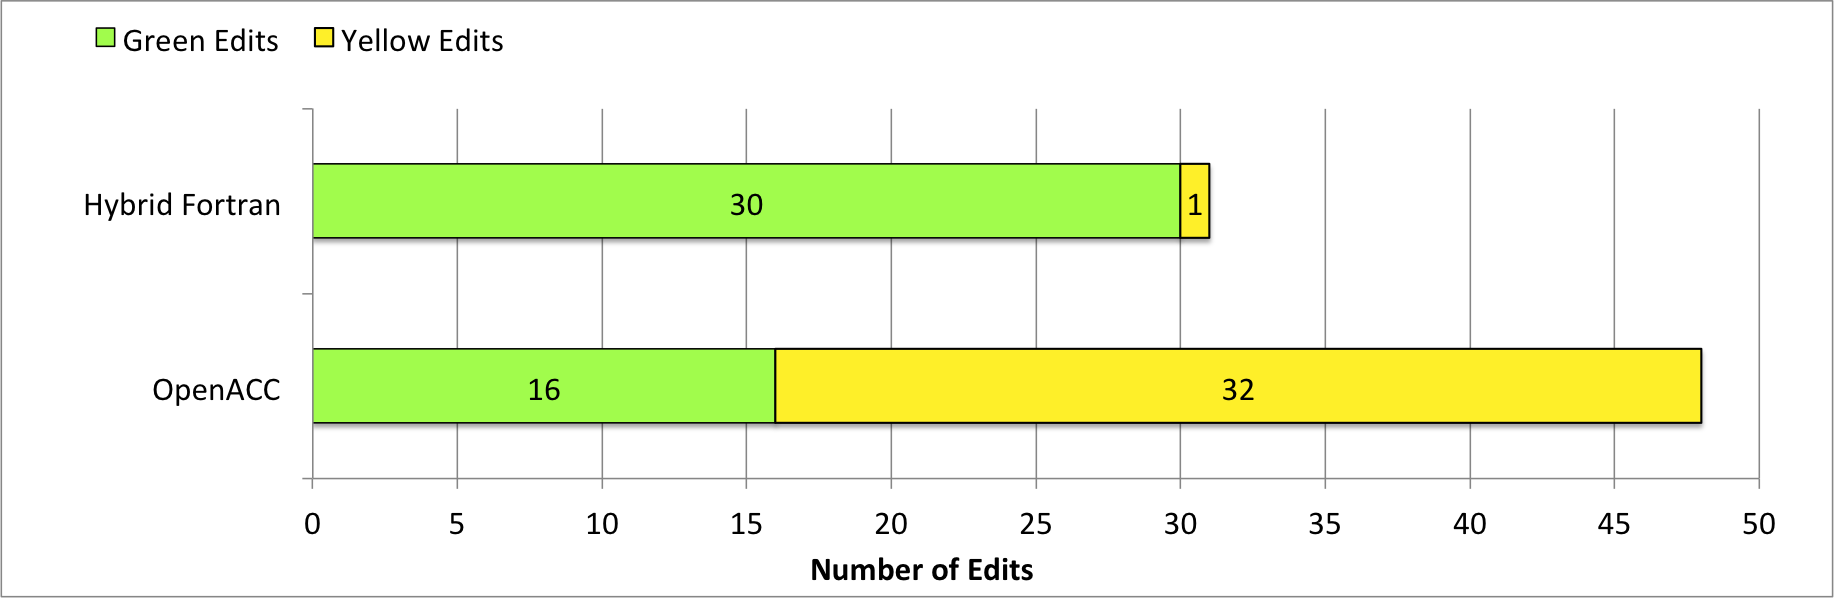
\includegraphics[width=14cm]{figures/verificationNumOfEdits}
        \caption[Usability Comparison]{Class and number of edits compared to original CPU code for ``setabssw'' kernel.}
        \label{figure:verificationNumOfEdits}
\end{figure}

Fig.~\ref{figure:verificationNumOfEdits} shows the results for the usability examination of sec.~\ref{sec:usabilityValidation}. Even though counting two find/replace operations as 14 edits, the \textbf{Hybrid Fortran} version still has a lower total number of edits than the OpenACC version. We can also see that the majority of code modifications are of the non problematic \textquotedblleft green\textquotedblright\ kind in the \textbf{Hybrid Fortran} case, while in the OpenACC version the majority of edits need to be applied more carefully.

We conclude that \textbf{Hybrid Fortran} is more easily applicable to the ASUCA physical core and it bears less potential for errors than OpenACC - an important aspect to keep in mind when doing GPU portations, since debugging on the GPU is not as straight forward as on the CPU, i.e. debugging for GPU has a higher cost in developer time.

\clearpage
\section{Performance of Hybrid Fortran} \label{sec:performanceValidation}

In this section the performance of \textbf{Hybrid Fortran} implemented code will be examined. The shortwave radiation module has been reused for that purpose, since benchmark implementations were already done using pure CUDA Fortran as well as OpenACC (see sec.~\ref{sub:testASUCARadSW}). In sec.~\ref{sub:performanceCPUValidation} we will examine the CPU performance, while sec.~\ref{sub:performanceGPUValidation} will show the GPU performance. All performance measurements have been repeated five times, the results shown here are averaged over those five runs. Again, only computation time is shown here, no host-to-device data copy time is being evaluated since the host-to-device bus performance is not expected to be relevant for the ASUCA GPU implementation.

\subsection{CPU Performance Comparison for Shortwave Radiation} \label{sub:performanceCPUValidation}
In this section we compare the CPU performance of the following implementations of the shortwave radiation (see also sec.~\ref{perfEvalShortwave}):

\begin{enumerate}
 \item Original CPU optimized code.
 \item OpenACC implementation compiled for CPU execution.
 \item Preprocessed CUDA Fortran implementation compiled for CPU execution.
 \item \textbf{Hybrid Fortran} implementation compiled for CPU execution.
\end{enumerate}

These implementations have been compiled using \verb|ifort -fast -openmp|\footnote{The Intel compiler tends to be very aggressive using the ``fast'' setting. This already enables the highest optimization settings as well as SSE vectorization. In general this has been found to perform well on the Intel hardware architecture used on TSUBAME 2.0.}. The OpenACC CPU implementation has additionally been compiled using \verb|pgf90|, since it has been found to perform poorly using the OpenACC agnostic \verb|ifort| compiler. The \verb|pgf90| compiler has for that reason been used with the following parameters\footnote{These settings have been carefully tested to perform well. Compiling the test module simply using ``pgf90 -fast -O4'' performs around 30\% worse than the settings shown here.}:

\begin{description}
 \item [-Mconcur] for enabling OpenMP multicore support.
 \item [-Mvect=sse] for enabling SSE vectorization support.
 \item [-Minline=levels:5,reshape] for enabling in-module-inlining for up to 5 levels including array parameter reshaping.
 \item [-O4] for enabling the most aggressive compiler optimizations.
 \item [-r8] for treating \verb|real| variables using double precision by default.
\end{description}

A few notes on the test settings:
\begin{enumerate}
 \item Concerning the multicore measurements: Since the parallel loops over \verb|IJ| are placed outside the radiation module for the original code version as well as the \textbf{Hybrid Fortran} CPU implementation, the execution time measurement for one submodule becomes non trivial in that case (thread synchronization would have to be used for the counters, which could have negative impact on the execution time itself). For that reason we have used the following approximation to measure the execution time of the shortwave radiation module in that case:
  \begin{enumerate}
  \item The ratio of shortwave radiation module execution time versus the overall test program execution time has been measured for all domain sizes in single core execution. These ratios have been found to be between 92\% and 95\% for all domain sizes for all test versions.
  \item These ratios have then been applied to the overall execution time in case of multicore execution.
  \end{enumerate}
 \item \verb|KIJ| storage order has been used for CPU execution for all test cases.
 \item Double precision arithmetics have been used for the computations.
\end{enumerate}

\begin{figure}[htpb]
        \centering
        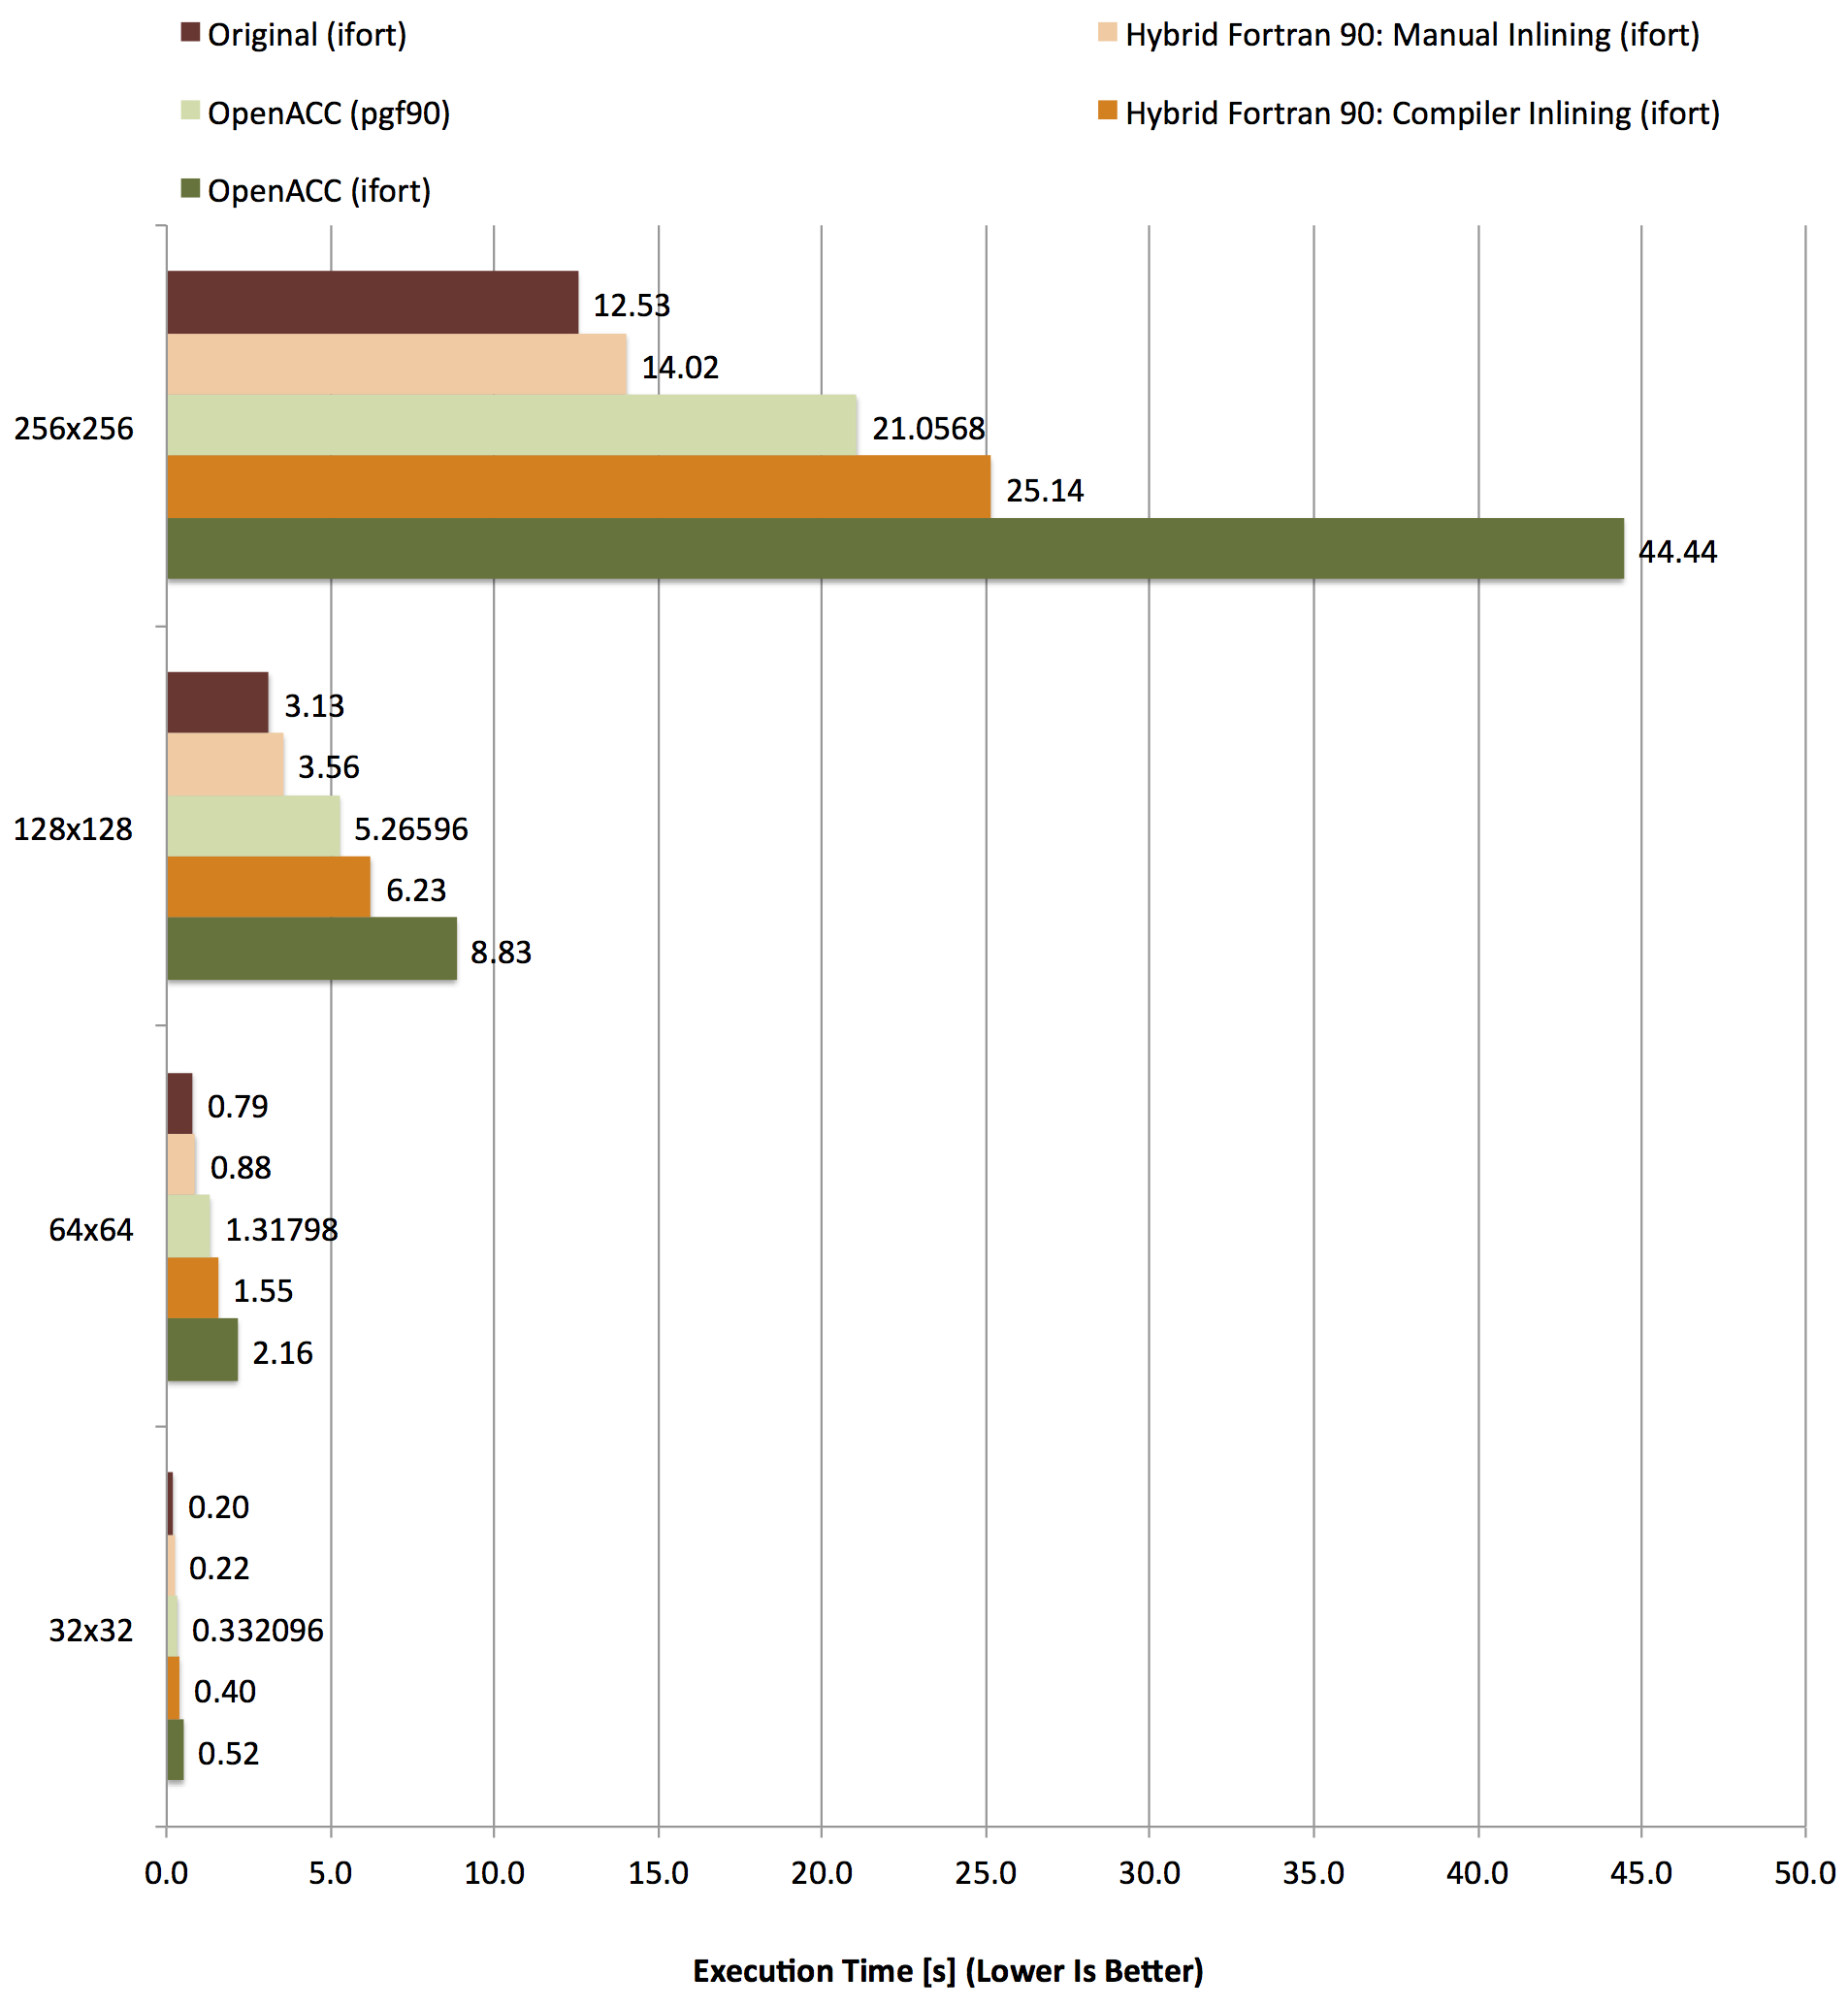
\includegraphics[width=14cm]{figures/verificationCPU1CoreExecTime}
        \caption[Single Core CPU Execution Time Results of Sample Implementation]{Single core CPU Execution time results for the ``radsw'' subprocedure grouped by grid sizes.}
        \label{figure:verificationCPU1CoreExecTime}
\end{figure}

Fig.~\ref{figure:verificationCPU1CoreExecTime} shows the single core execution time results on CPU. The following performance characteristics can be examined from these results:
\begin{enumerate}
 \item As expected the execution time is proportional to the area of the \verb|IJ| domain.
 \item The shortwave radiation module performance has been found to be heavily dependant on the inlining method being used. As a GPU optimization some scalar subroutines have been introduced (see fig.~\ref{figure:asucaPPImplementationCPU} in sec.~\ref{sec:asucaRadImplementation}) for the \textbf{Hybrid Fortran} version. Trying to inline these with the \verb|ifort| compiler has proven to be difficult, hence a manually inlined version was implemented as well, essentially recreating the same code as in the original version. Doing so lead to an improvement of factor 1.8 in CPU performance, giving the \textbf{Hybrid Fortran} version almost the same performance characteristics as the original CPU version.
 \item Curiously, \verb|ifort| compiled OpenACC code performs more than 200\% worse than the \verb|pgf90| compiled version. One could suspect that \verb|ifort| is more dependant on the loop structure being optimized for CPU. In all preliminary tests for the original code version as well as \textbf{Hybrid Fortran} CPU implementations, \verb|ifort| has performed at least 30\% better than \verb|pgf90|. For the following tests we therefore concentrated on \verb|pgf90| for the OpenACC CPU implementations while keeping \verb|ifort| for all other CPU implementations.
 \item The OpenACC version has also continually been optimized, both through compiler settings and preprocessor directives for the reordering of the inner loops of the \verb|radsw| subroutine (i.e. the order of the spectral loop and the parallel \verb|IJ| loops has been optimized for CPU as well as GPU). Also, the OpenACC version is already fully inlined, which has been found to be optimal for CPU execution. Nevertheless we were unable to come close to the original CPU execution times using the OpenACC program structure. This was expected, however, because of the loop structure target conflict explained in sec.~\ref{sub:swDivertingGoals}.
\end{enumerate}

\begin{figure}[htpb]
        \centering
        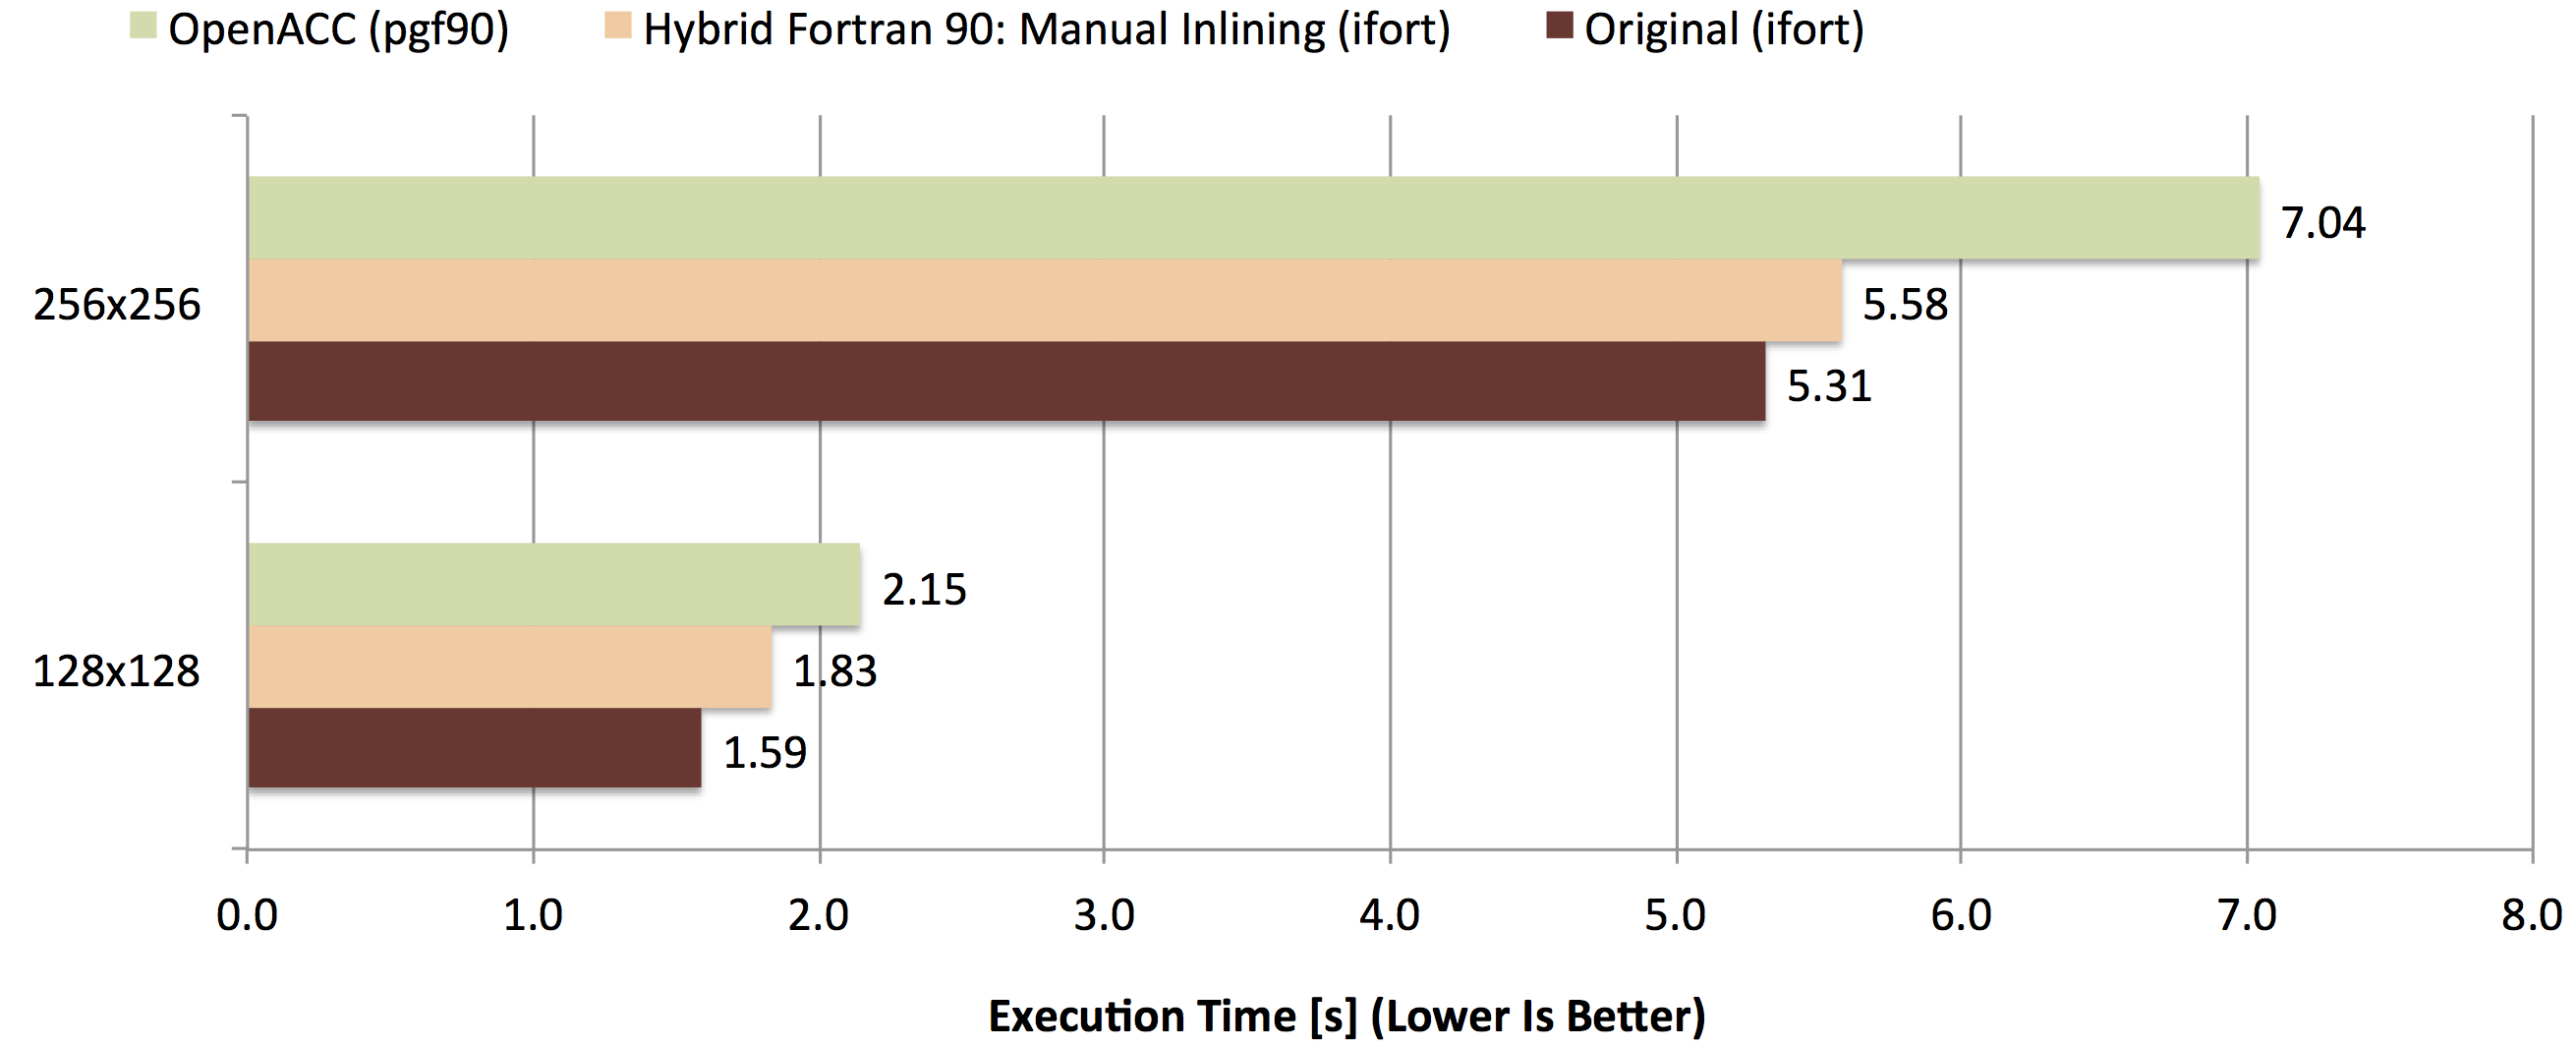
\includegraphics[width=14cm]{figures/verificationCPU6CoreExecTime}
        \caption[Six Core CPU Execution Time Results of Sample Implementation]{Six core CPU Execution time results for the ``radsw'' subprocedure grouped by grid sizes.}
        \label{figure:verificationCPU6CoreExecTime}
\end{figure}

Fig.~\ref{figure:verificationCPU6CoreExecTime} shows the six core execution time results on CPU. For the multicore tests we have used the best performing version of both \textbf{Hybrid Fortran} and OpenACC. In case of OpenACC, the OpenMP directives for multicore execution have been added at the same place as the OpenACC accelerator directives (which are omitted for CPU compilation). We can see that this leads to very similar results as the single core case shown before - however the differences are less pronounced. This is to be expected since the shortwave radiation submodule is less computationally bound on multicore execution in comparison to single core execution, which hides computational inefficiencies (see also sec.~\ref{sub:swCharacteristics}). The performance loss graphs in fig.~\ref{figure:verificationLossVS1Core} and fig.~\ref{figure:verificationLossVS6Core} also show this characteristic.

Overall it becomes clear that complex OpenACC code portations can at best be expected to loose between 30\% and 60\% when executed on CPU, even after optimizations. The \textbf{Hybrid Fortran} version that has been automatically adjusted for the CPU, remarkably only shows 5\% loss at best, 16\% at the most. In other words, using \textbf{Hybrid Fortran} instead of OpenACC has been found to result in an improvement from 26\% up to 50\% in CPU execution time - a remarkable achievement.

\begin{figure}[htpb]
        \centering
        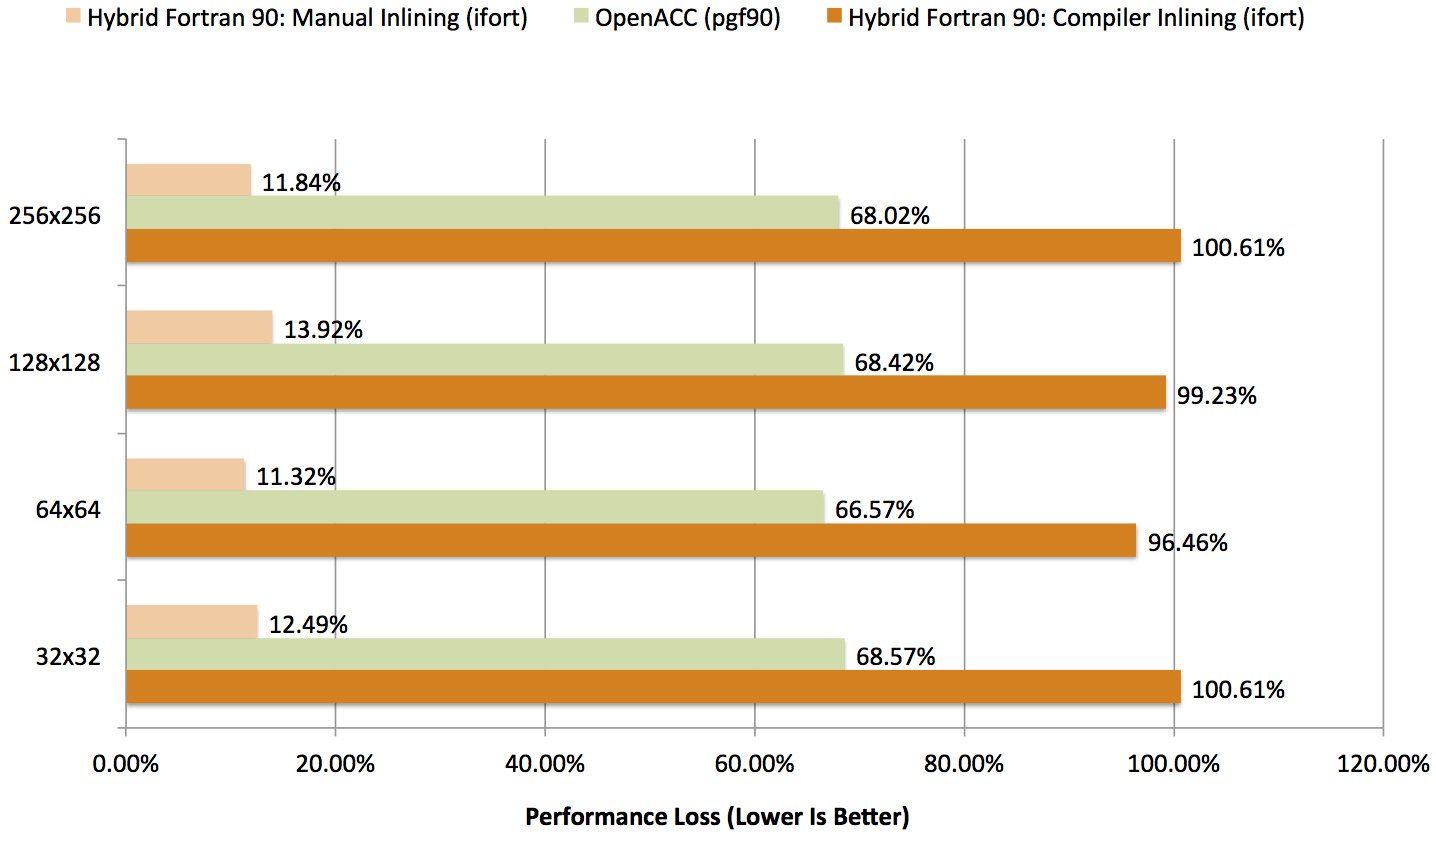
\includegraphics[width=14cm]{figures/verificationLossVS1Core}
        \caption[CPU Single Core Performance Loss of Sample Implementation]{Performance loss for the ``radsw'' kernel on single core CPU (compared to original CPU code compiled with ``ifort'') grouped by grid sizes.}
        \label{figure:verificationLossVS1Core}
\end{figure}

\begin{figure}[htpb]
        \centering
        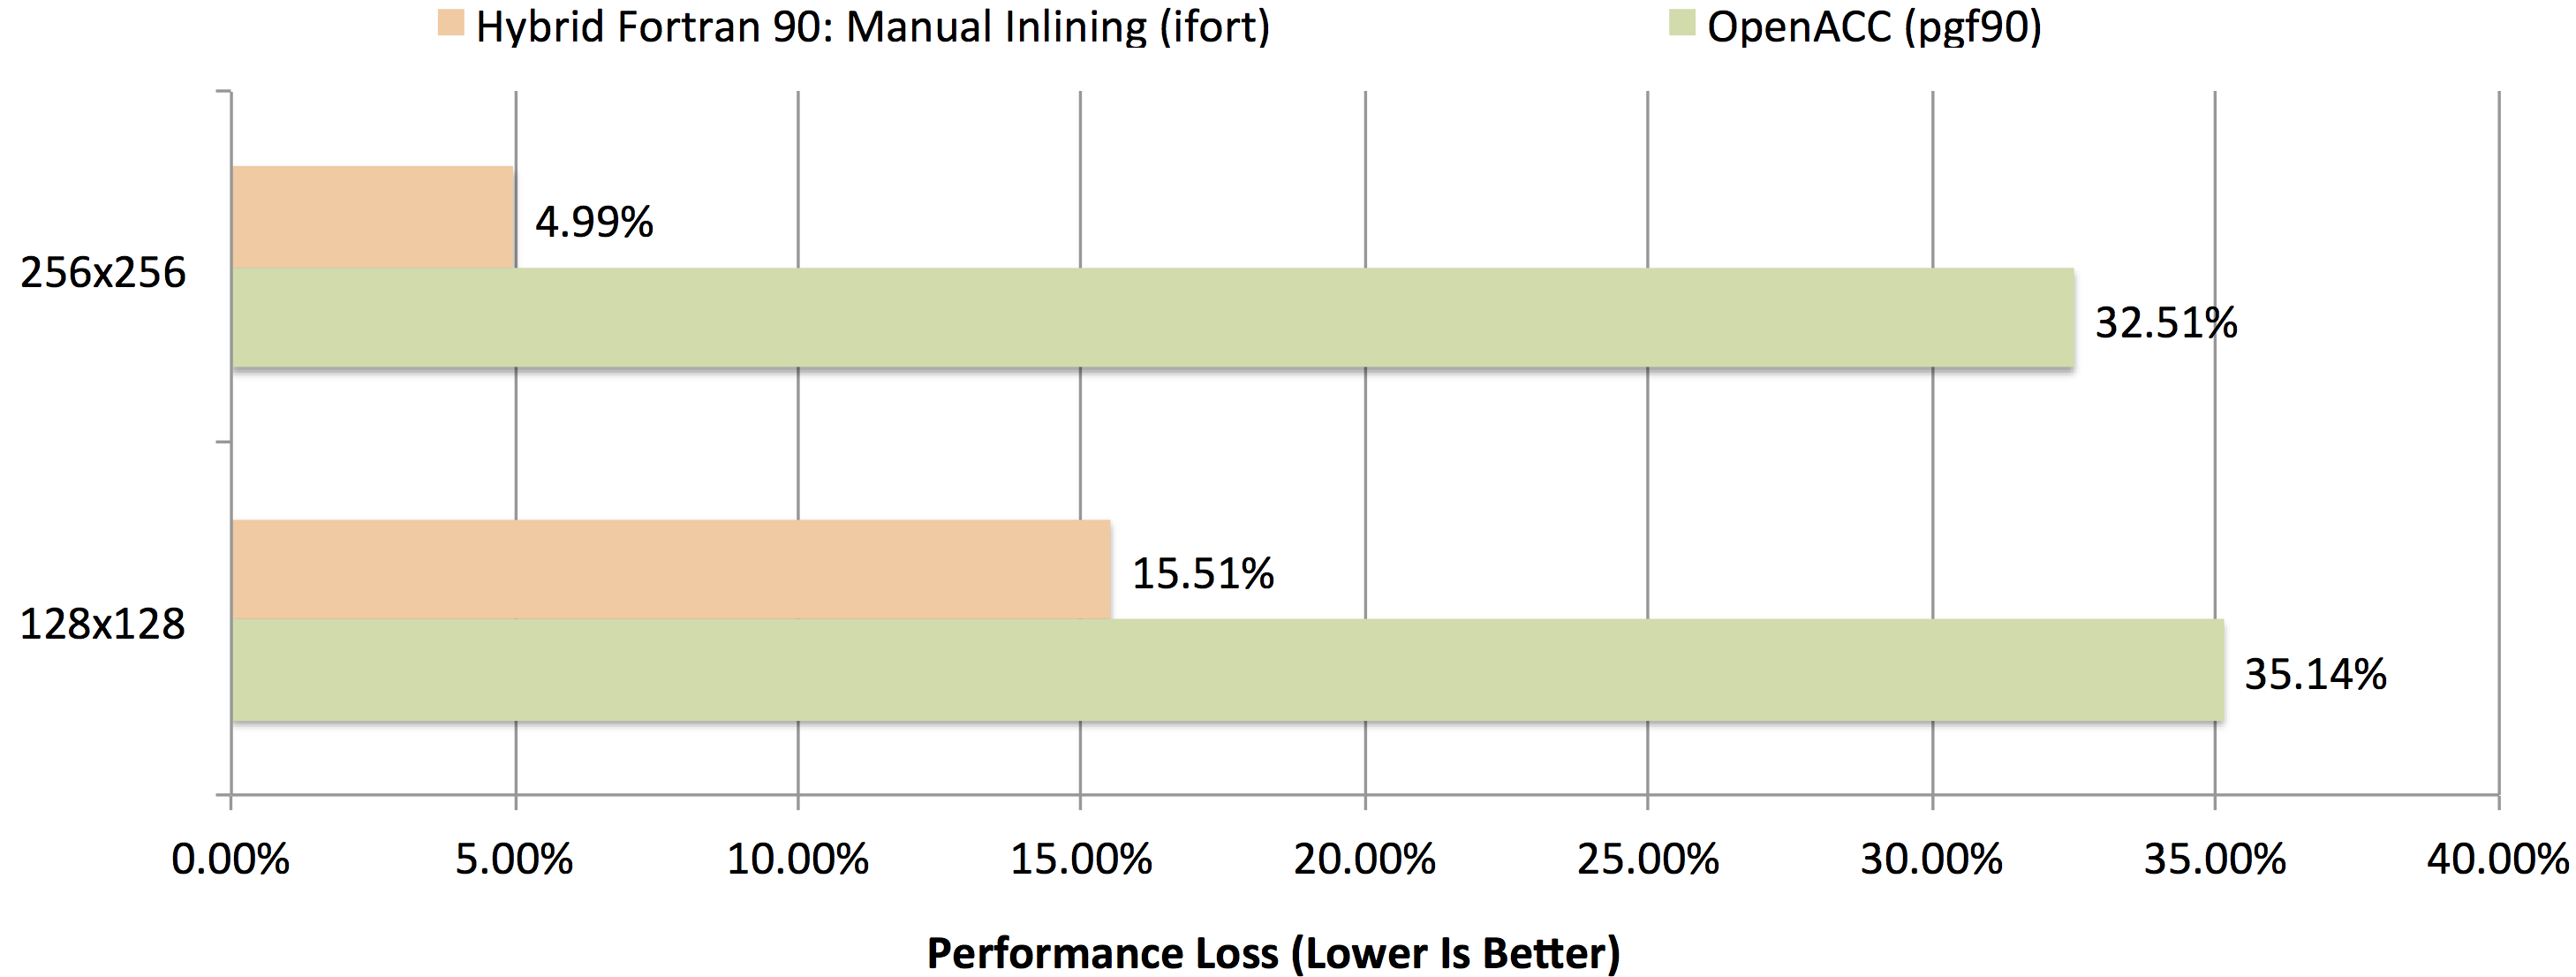
\includegraphics[width=14cm]{figures/verificationLossVS6Core}
        \caption[CPU Six Core Performance Loss of Sample Implementation]{Performance loss for the ``radsw'' kernel on six core CPU (compared to original CPU code compiled with ``ifort'') grouped by grid sizes.}
        \label{figure:verificationLossVS6Core}
\end{figure}

\clearpage
\subsection{GPU Performance Comparison for Shortwave Radiation} \label{sub:performanceGPUValidation}

In terms of GPU performance we compare the \textbf{Hybrid Fortran} version with the PGI OpenACC version as well as a preliminarily implemented CUDA Fortran version referred to as \textquotedblleft Preprocessed CUDA Fortran\textquotedblright, see also sec.~\ref{perfEvalShortwave}.

Some notes on the settings:
\begin{enumerate}
 \item \verb|IJK| storage order has been used throughout here, which is optimal for GPU execution.
 \item The same compiler settings as introduced in sec.~\ref{sub:openACC} have been used for the OpenACC version.
 \item The same compiler settings as introduced in sec.~\ref{sub:cudaFortran} have been used for the CUDA Fortran and \textbf{Hybrid Fortran} GPU versions.
 \item As all other tests with shortwave radiation, this comparison has been done using double precision arithmetics.
\end{enumerate}

\begin{figure}[htpb]
        \centering
        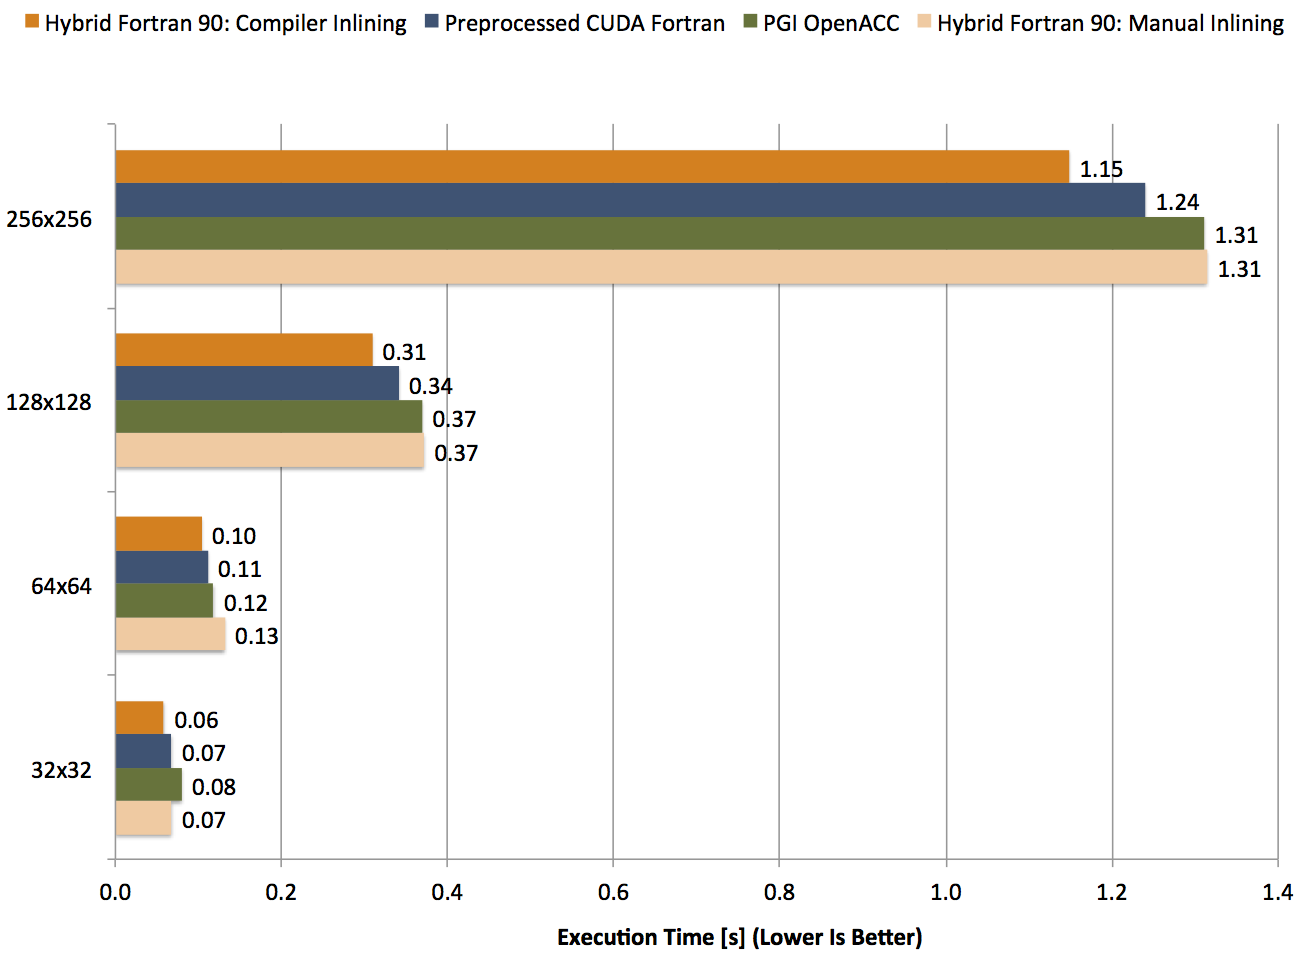
\includegraphics[width=14cm]{figures/verificationGPUExecTime}
        \caption[GPU Execution Time Results of Sample Implementation]{GPU Execution time results for the ``radsw'' kernel grouped by grid sizes.}
        \label{figure:verificationGPUExecTime}
\end{figure}

Fig.~\ref{figure:verificationGPUExecTime} shows the execution time results on GPU. We can make the following observations:
\begin{enumerate}
 \item From $32\times32$ to $128\times128$ \verb|IJ| domain sizes the execution time scales under proportional to the \verb|IJ| area. This is an expected behaviour on NVIDIA GPUs as their scheduler can make better use of the available bandwidth as well as computational ressources with a higher number of threads. Between $128\times128$ and $256\times256$ the performance appears to saturate. Fig.~\ref{figure:verificationSpeedupVS1Core} shows this behaviour more clearly in terms of speedup.
 \item \textbf{Hybrid Fortran} with manual inlining shows the same GPU performance as the PGI OpenACC version - an interesting result, since those two versions are very similar in their code structure in terms of loop positioning. This shows that PGI OpenACC performs well on the GPU for bandwidth limited problems (which holds true for shortwave radiation executed on GPU, see also sec.~\ref{sub:swCharacteristics}).
 \item Using the new scalar subroutines inside the \verb|radsw| kernel and letting them be inlined by \verb|nvcc| (which is at the base of the CUDA Fortran compiler being used), the \textbf{Hybrid Fortran} version is able to gain another 14\%. We expect different register allocation behaviour on the GPU depending on code inlining to be the reason for this characteristic. We have therefore introduced preprocessor directives to switch between manual inlining and compiler inlining depending on whether the code is compiled for GPU or CPU - we consider this to be still a fair comparison however, since the OpenACC code has been optimized using preprocessor directives as well.
 \item Compared to the hand-implemented CUDA Fortran version, the \textbf{Hybrid Fortran} gains 8\% in speed. We expect a reduction in branches inside the \verb|radsw| kernel to be the reason - this optimization has been found while implementing the \textbf{Hybrid Fortran} version thanks to increased familiarity with the codebase.
 \item In sec.~\ref{sub:hardwareSystemBalance} a speedup of $11.1\times$ versus single core and $5.3\times$ versus six core CPU execution was estimated for memory bandwidth limited problems. The best results (by the \textbf{Hybrid Fortran} GPU version) shown in fig.~\ref{figure:verificationSpeedupVS1Core} and fig.~\ref{figure:verificationSpeedupVS6Core} are all within 15\% of those values for the saturated case, even within 1.5\% in the speedup versus single core execution. This shows that
  \begin{enumerate}
   \item The hardware model introduced in sec.~\ref{sub:hardwareSystemBalance} is very reasonable for memory bandwidth limited problems.
   \item The \textbf{Hybrid Fortran} GPU implementation for shortwave radiation is close to the optimum performance that can be achieved, validating the capabilities of this framework.
  \end{enumerate}
\end{enumerate}

Overall the GPU performance of the compared approaches is relatively similar in this bandwidth limited case. CUDA Fortran implementations (both implemented by hand and implemented automatically by using the new \textbf{Hybrid Fortran} framework) do perform between 5\% and 15\% better than PGI OpenACC - a similar result has been found for the simple 3D Diffusion test shown in sec.~\ref{sec:perfEvalDiffusion} where PGI OpenACC performed on par with CUDA C as well. For computationally bound problems however we would expect a much more significant advantage for CUDA code versions based on the results of the Particle Push, shown in sec.~\ref{sec:perfEvalParticle}, where CUDA C was found to perform $2.3\times$ faster than PGI OpenACC.

\begin{figure}[htpb]
        \centering
        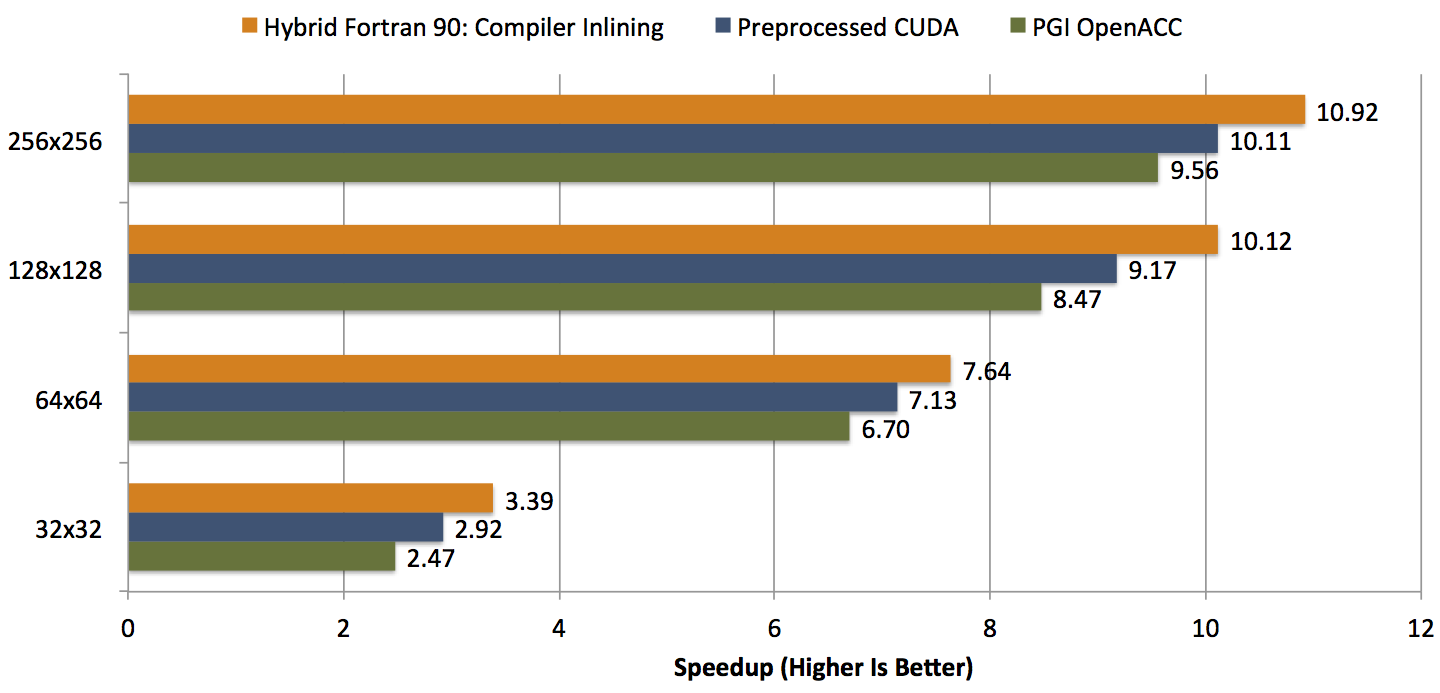
\includegraphics[width=14cm]{figures/verificationSpeedupVS1Core}
        \caption[GPU Speedup Results of Sample Implementation Compared to Single Core]{GPU Speedup results for the ``radsw'' kernel compared to single core CPU (ifort) grouped by grid sizes.}
        \label{figure:verificationSpeedupVS1Core}
\end{figure}

\begin{figure}[htpb]
        \centering
        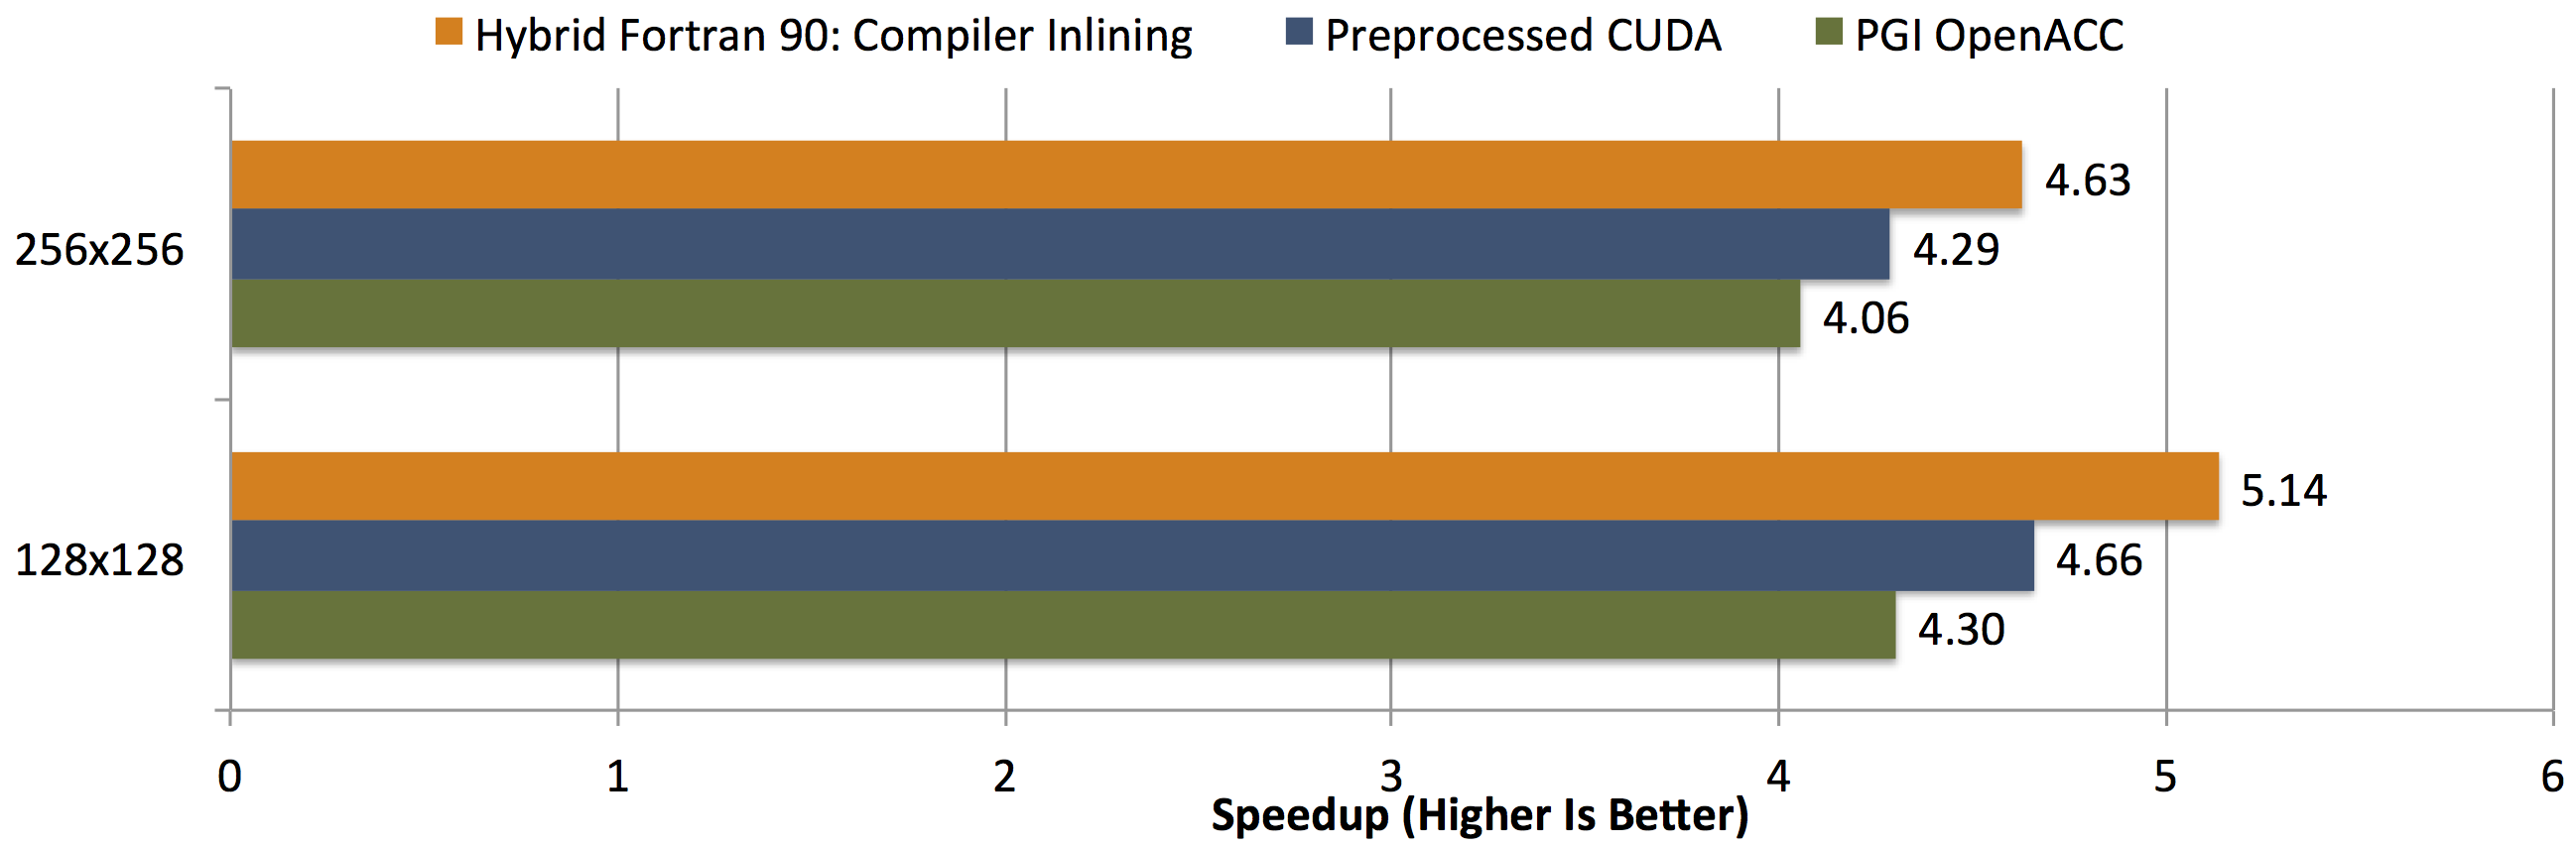
\includegraphics[width=14cm]{figures/verificationSpeedupVS6Core}
        \caption[GPU Speedup Results of Sample Implementation Compared to Six Core]{GPU Speedup results for the ``radsw'' kernel compared to six core CPU (ifort) grouped by grid sizes.}
        \label{figure:verificationSpeedupVS6Core}
\end{figure}

% \clearpage
% \subsection{Overall Performance of New Radiation Module} \label{sub:performanceOverallValidation}
%

% I have found some new results when analyzing the CPU behavior of the ported shortwave code. 
%
% My biggest finding was, that the Intel Fortran compiler is actually massively faster for the original code compared to PGI, it is about a factor of 2x (pink vs. light blue in top graph)! The hybridized code had trouble catching up to this (green, top graph). I've found that the innermost subprocedure calls in the hot loop were responsible (these have been introduced as a GPU optimization). The compiler-inlining just didn't work well with those, I suspect that the inlining creates unnecessary temporary scalars for the inlined function parameters. Manually inlining those subprocedures in the hybrid code resulted in a CPU version almost as fast as the original (still about 10\% loss). I suspect that it would be very hard for the OpenACC CPU version to catch up, since the difference of this implementation to the original is massive (which can be regarded as a success for they Hybrid Fortran framework, since it allows CPU code very close to the original, fully optimized version). 
%
% Now for the GPU version the opposite is true: The manually inlined code performs about 10-15\% worse than the compiler inlined version (red vs. blue in the middle graph). NVCC seems to be more optimized for compiler inlining since this functionality is essential for GPU code. With the new manually inlined implementation the GPU code of Hybrid Fortran and OpenACC are on par. 
%
% Conclusion: In order to get the last 20]\% out of both CPU and GPU code, it is either necessary to make use of conditional compilation OR the Hybrid Fortran framework would have to be adapted. In the case shown here, a custom inlining module as part of the framework would be useful, but sadly not possible in the timeframe of this master thesis. In any case the Hybrid Fortran framework performs either equal or better than OpenACC however. 
%
% \section{Memory Boundedness vs. Computational Boundedness}
%
%
% what is arithmetic intensity?
%
% double precision -> hard to predict arithmetic intensity on GPU for a big kernel because of software implementation of operations -> cite CUDA reference. same applies to CPU.
%
% -> use empirical profiling, check feasibility of results with later performance results.
%
% cpu + gpu
%
% -> we see: memory bandwidth limited
%
% \section{Memory Bandwidth Model}
%
% special case: no stencil computations without memory accesses at offset in i, j- direction. assume perfect caching and access of in- arrays, out-arrays once at every place. inout = twice. -> ideal model
%
% memory bandwidth CPU = ?
%
% memory bandwidth GPU = ?
%
% \section{Execution Time Analysis} \label{sec:execTimeAnalysis}
% memory bound - should be proportional to memory bandwidth
%
% analysis of inlining behaviour
%
% manual vs compiler inlining
% OpenACC on CPU pgf90 vs ifort
%
%
% \subsection{CPU Execution}
%
% OpenACC vs handmade hybrid CUDA Fortran vs generated hybrid CUDA Fortran
%
% \subsection{GPU Execution}
%
% \section{Conclusion}